\documentclass[review]{elsarticle}

\makeatletter
\def\@author#1{\g@addto@macro\elsauthors{\normalsize%
    \def\baselinestretch{1}%
    \upshape\authorsep#1\unskip\textsuperscript{%
      \ifx\@fnmark\@empty\else\unskip\sep\@fnmark\let\sep=,\fi
      \ifx\@corref\@empty\else\unskip\sep\@corref\let\sep=,\fi
      }%
    \def\authorsep{\unskip,\space}%
    \global\let\@fnmark\@empty
    \global\let\@corref\@empty  %% Added
    \global\let\sep\@empty}%
    \@eadauthor={#1}
}
\makeatother

\usepackage{lineno}
\usepackage{color}
\usepackage[hidelinks]{hyperref}
\usepackage{graphicx}
\usepackage{caption}
\usepackage{epstopdf}
\usepackage{multirow}
\usepackage{lineno}
\usepackage{amssymb}
\usepackage{pgfplots}
\usepackage{tikz}
\usepackage{subcaption}
\usepackage{rotating}
\usepackage{threeparttable}
\usepackage{setspace}
\usetikzlibrary{matrix}
\usetikzlibrary{spy}
\usepgfplotslibrary{groupplots}
\pgfplotsset{compat=newest}
\graphicspath{ {./figures/} }



\modulolinenumbers[5]
\journal{Journal of \LaTeX\ Templates}

%%%%%%%%%%%%%%%%%%%%%%%
%% Elsevier bibliography styles
%%%%%%%%%%%%%%%%%%%%%%%
%% To change the style, put a % in front of the second line of the current style and
%% remove the % from the second line of the style you would like to use.
%%%%%%%%%%%%%%%%%%%%%%%

%% Numbered
%\bibliographystyle{model1-num-names}

%% Numbered without titles
%\bibliographystyle{model1a-num-names}

%% Harvard
%\bibliographystyle{model2-names.bst}\biboptions{authoryear}

%% Vancouver numbered
%\usepackage{numcompress}\bibliographystyle{model3-num-names}

%% Vancouver name/year
%\usepackage{numcompress}\bibliographystyle{model4-names}\biboptions{authoryear}

%% APA style
%\bibliographystyle{model5-names}\biboptions{authoryear}

%% AMA style
%\usepackage{numcompress}\bibliographystyle{model6-num-names}

%% `Elsevier LaTeX' style
\bibliographystyle{elsarticle-num}
%%%%%%%%%%%%%%%%%%%%%%%

\begin{document}
\doublespacing
%\Large
%\setstretch{1.1}


\begin{frontmatter}

\title{Barrelling formation during the axial compressive experiments on cubic
samples with  isotropic, transversely isotropic and orthotropic elastic
properties {\color{red} Preliminary title}}
%%\tnotetext[mytitlenote]{Fully documented templates are available in the
% elsarticle package on \href{http://www.ctan.org/tex-archive/macros/latex/contrib/elsarticle}{CTAN}.}

%% Group authors per affiliation:






%%\fntext[fn1]{This is the specimen author footnote.}
%%\fntext[fn2]{Another author footnote, but a little more longer.}
%%\fntext[fn3]{Yet another author footnote. Indeed, you can have any number of
% author footnotes.}
\cortext[cor1]{Corresponding author}
\author{Alexey Vorobyev\corref{cor1}}
\ead{alexey.vorobyev@me.com}


\author{Ingela Bjurhager}
\author{Nico P. van Dijk}
\author{Kristofer Gamstedt}

\address{Uppsala University, Division of Appplied Mechanics,
Uppsala, Sweden }



\begin{abstract}
For scarce materials, such as archaeological wood, one often resorts to cubic
samples instead of standardised prisms for mechanical tests. For these samples
barreling formation gives rise to additional difficulties difficulties in
identifying the elastic properties.
Furthermore natural orthotropy, availability and variation between and within
samples make the mechanical characterisation of wood  challenging. 
The purpose of the present study is to experimentally and numerically investigate the effects of barrelling
formation in cubic samples during compressive experiments. Secondly, to investigate and
compare barrelling formation on isotropic, transversely 
isotropic and orthotropic material parameters. \par
Finally to compare four strain measurement techniques using
Digital Image Correlation (DIC), strain gauges and direct
reading from of universal testing mashine and investigate which is better for
quantification of mechanical parameters such as Young's moduli and Poisson's ratios.
The elastic parameters determined from the simulated tests were normalised with regards to the input parameters. The presented relative errors provide information when the perturbation caused by barreling effect is negligible or significant for various materials and strain measurements. 
As an example, compressive tests on waterlogged archaeological oak impregnated
with polyethylene glycol (PEG) are discussed.


\end{abstract}

\begin{keyword}
Cubic samples\sep Compressive testing\sep Barrelling formation \sep
Wood
\end{keyword}

\end{frontmatter}

\linenumbers

\section{Introduction}

Characterisation of material stiffness properties of orthotropic materials can
be challenging. In  careful design of wood structures, not only one parameter, but the full
orthotropic set of elastic parameters is needed \cite{tsoumis1991science},
e.g. for finite-element modelling of wood joints that are locally subjected to a
triaxial stress state. Compressive experiments are generally considered to be
reliable method for identifying engineering constants such as Young's moduli and Poisson's ratios. The general approach is to measure the material response due to applied
forces. The procedure is straightforward and easy to perform due to simplicity of experimental installation and low requirements to sample
geometry. ASTM D143 standard \cite{standard1997d143,
johnson1983compression} require the usage of elongated rectangular prisms for
the compressive testing along with strain gauges.
For rare materials such as archaeological wood, it is more convenient to use
cubic samples \cite{ljungdahl2007transverse, vorobyevcharacterisation} to save
material.
This enables the same sample to be tested several times and in
different directions (typically radial, tangential, longitudinal) if the loads are
applied within the elastic range and do not cause and irreversible damage in the material.
A disadvantage of compressive testing of cubes compared to the tensile testing
of dog-bone samples is that it can be difficult to ensure a homogeneous stress
state due to geometrical imperfections in the test samples
\cite{Toftegaard1999849}.
Moreover, barrelling  (as illustrated in Figure \ref{fig:barrelling}) during
compressive loading \cite{oldroyd1966stress} caused by friction between the platens and the
sample makes it difficult to assess the non-uniform deformation in order to determine the elastic paramters.
Consequently, the Poisson's ratios cannot be obtained directly under such constraints. 
The classical way to measure strain is by using the loading platen position or electrical-resistance strain gauges. Nowadays, full field strain measurement techniques such
as digital speckle photography (DSP) \cite{synnergren1999stereoscopic} and
3D/stereo-digital image correlation (DIC) \cite{majano2012test} are 
increasingly being used.The strain-field measurement technique using
DIC has been shown advantages in comparison with the traditional strain gauges
\cite{huang2010optical,xavier2012stereovision}. In particular, full-field measurements can help to improve the estimation of the stiffness parameters \cite{dahl2009planar,
majano2012test, ozyhar2013moisture}. 
Despite technical difficulties in obtaining accurate elastic properties by compressive testing of wooden cubes, it is still a reasonable 
choice of test method if the amount of available material is limited, as is the case for e.g.\ archaeological material. The intention of the present work is to estimate how large the measurement errors can due to the inevitable barrelling effect, and which strain measures are suitable to reduce such errors.  \par 

This study was initiated when in order to better estimate the stiffness properties of water-logged and preservation-treated  oak of the Vasa shipwreck, displayed at a public museum in Stockholm. The stiffness of the material is needed as input parameters in a finite-element model of the ship, which can be used in the design of a future improved support system for the ship. The Vasa capsized in 1628, and was salvaged in 1961. 
The waterlogged ship was impregnated with polyethylene glycol (PEG) in an extensive conservation process aiming to prevent deformation during drying. 
Extensive research during the last decades have shown that the ship is suffering
from aggressive chemical degradation. Both the degradation \cite{bjurhager2012state}
and the PEG impregnation \cite{ljungdahl2007transverse} have had a negative effect on the mechanical properties of the ship, which is in need of a better support. \par
Previously compressive experiments on prismatic samples with orthotropic
material behavior were simulated by Toftegaard \cite{Toftegaard1999849} who investigated the effect of geometrical imperfections on the
engineering elastic constants.
In his work Toftegaard compared the simulated strain field to the measurements
of strain gauges and obtained good agreement between the simulated and experimental
data.\par
In the present work, DSP has been used in order to obtain the experimental
strain field, based on the displacement field over an area rather than locally
at metallic foil pattern of a strain gauge.
Chen \cite{Chen001} simulated the deformation behaviour of samples with geometrical
imperfections supported by a locked hemispherical seat compared to conventional platens. This is useful for rigid platens which cannot adjust to sample geometry to spread the loads more evenly over the contact area.
\par 

%The purpose of experiment



The purpose of the present work is to investigates the occurence of barrelling
 on the accuracy of the obtained elastic properties in three different types of material behaviour, namely isotropic, transversely isotropic and orthotropic elastic properties, in ranges applicable for archeological wood.
Additionally, four strain measuring techniques using DSP (full field and central
area of interest), strain gauges (recommended by the standard 
\cite{standard1997d143, johnson1983compression}) and direct compressive platen
displacement measurement are compared in order to assess the magnitude of the
resulting errors.
The results can help to estimate the induced errors for the alternative strain measurement methods. 
% 
% This enables testing of the same sample several times and in
% different directions (radial, tangential, longitudinal) if the loads are
% applied within the elastic range.
% A disadvantage with compressive testing of cubes compared to tensile testing of
% dog-bone specimens, is that it can be complicated to ensure a homogeneous stress state
% due to geometrical imperfections of test specimens \cite{Toftegaard1999849}.
% Moreover, barrelling formation (Figure \ref{fig:barrelling}) in compressive
% loading \cite{oldroyd1966stress}, due to friction between the platens and the
% sample, makes it difficult to assess the  deformations.
% Consequently, the Poisson's ratios are thus more difficult to obtain directly from this kind
% of loading.
% The conventional way to measure strains is by using the built in measurement
% system or strain gages. Nowadays, full field strain measurement techniques such
% as digital speckle photography (DSP) \cite{synnergren1999stereoscopic} and
% 3D/stereo-digital image correlation (DIC) \cite{majano2012test} are used more
% and more. Strain field measurements technique using DIC has shown a good
% performance in comparison to the traditional strain gauges
% \cite{huang2010optical,xavier2012stereovision} Additionally it helps to
% improve the estimation of the stiffness parameters \cite{dahl2009planar,
% majano2012test, ozyhar2013moisture}. 
% Nevertheless, compressive testing of wooden cubes is the reasonable 
% choice of test method if the amount of available material is limited, as is the case for archaeological material.\par 
% 
% In 2012, a project with the aim of designing a new support structure for the
% archaeological Vasa ship was initiated. The ship was capsized in 1628, and was salvaged in 1961. 
% The waterlogged ship was impregnated with polyethylene glycol (PEG) in an extensive conservation process aiming to prevent deformation during drying. 
% Extensive research during the last decades have found that the ship suffers from
% aggressive chemical degradation. Both the degradation \cite{bjurhager2012state}
% and the PEG impregnation \cite{ljungdahl2007transverse} have had a negative effect on the mechanical properties of the ship, which is in need of a better support. In 2012 a project with the aim of 
% designing a new support structure for the fragile and soft ship was also initiated. For this task, the elastic, ultimate and creep properties of the 
% Vasa oak need to be determined. Due to the limited access to material, cubic samples which can be tested several times is preferred.
% In order to verify the results from the compressive experiments the effect of
% barrelling was investigated by the simulation using the Finite Element
% Modelling (FEM).\\
% Previously compressive experiments on prism samples with orthotropic material
% behavior were simulated by Toftegaard \cite{Toftegaard1999849} in order to
% investigate the effect of geometrical imperfections on identification of
% engineering elastic constants.
% in his work he compared the simulated strain field to the measurements of strain
% gauges and obtained good agreement between the simulated data and experimental
% curves.\par
% The present work uses DSP in order to obtain the experimental strain field,
% based on the displacements in an area rather than two points using a strain
% gauge.
% Chen \cite{Chen001} has simulated the behaviour of specimens with geometrical
% imperfections on a locked  seat during the compressive experiments
% of composite materials. This is relevant when the platens of universal testing
% machine are locked and cannot adjust to sample geometry.
% When a prism specimen is compressed between platens it expand transversely.
% Its surfaces bear heterogeneous deformation that are resulting in barreling
% formation of the prism.\par 
% 
% % %The purpose of experiment
% 
% 
% 
% The present work investigates
% barrelling formation in three different types of material behaviour.
% Additionally three strain measuring techniques using DSP and strain gauges are
% compared in order to identify the magnitude of resulting errors.
% The results can help to identify the accuracy of the material constants values
% of elastic parameters that can be obtained during compressive experiments on
% cubic samples.


\section{Materials and Methods}

\begin{figure}
    \centering
    \begin{subfigure}[b]{0.4\textwidth}
        \centering
        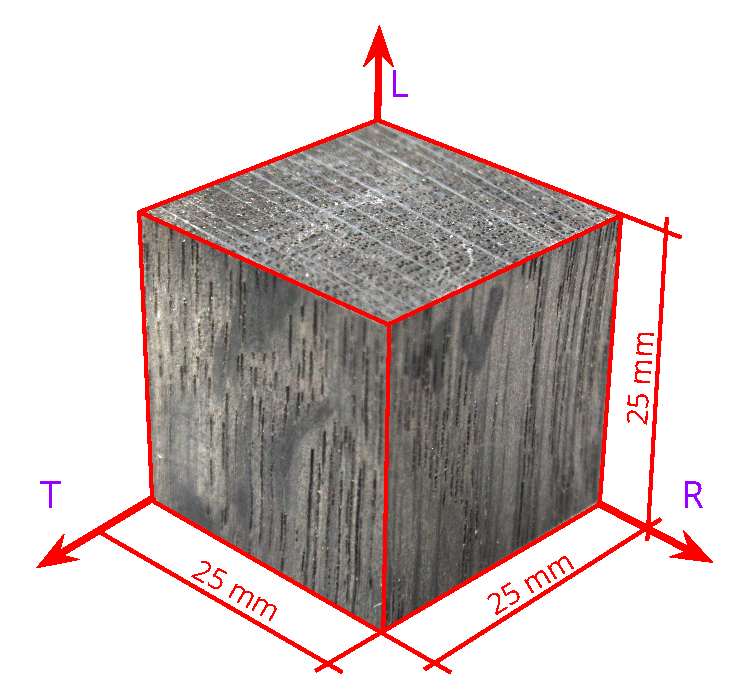
\includegraphics[width=\textwidth]{VasaCube.pdf}
        \caption{}
        \label{fig:vasacube}
    \end{subfigure}
    \hfill
    \begin{subfigure}[b]{0.4\textwidth}
        \centering
        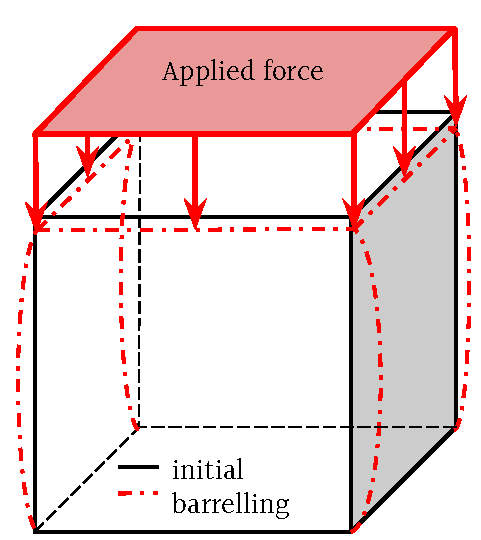
\includegraphics[width=\textwidth]{BarellingEffectZoomed.pdf}
        \caption{}
        \label{fig:barrelling}
    \end{subfigure}
    \hfill
    \begin{subfigure}[b]{0.4\textwidth}
        \centering
        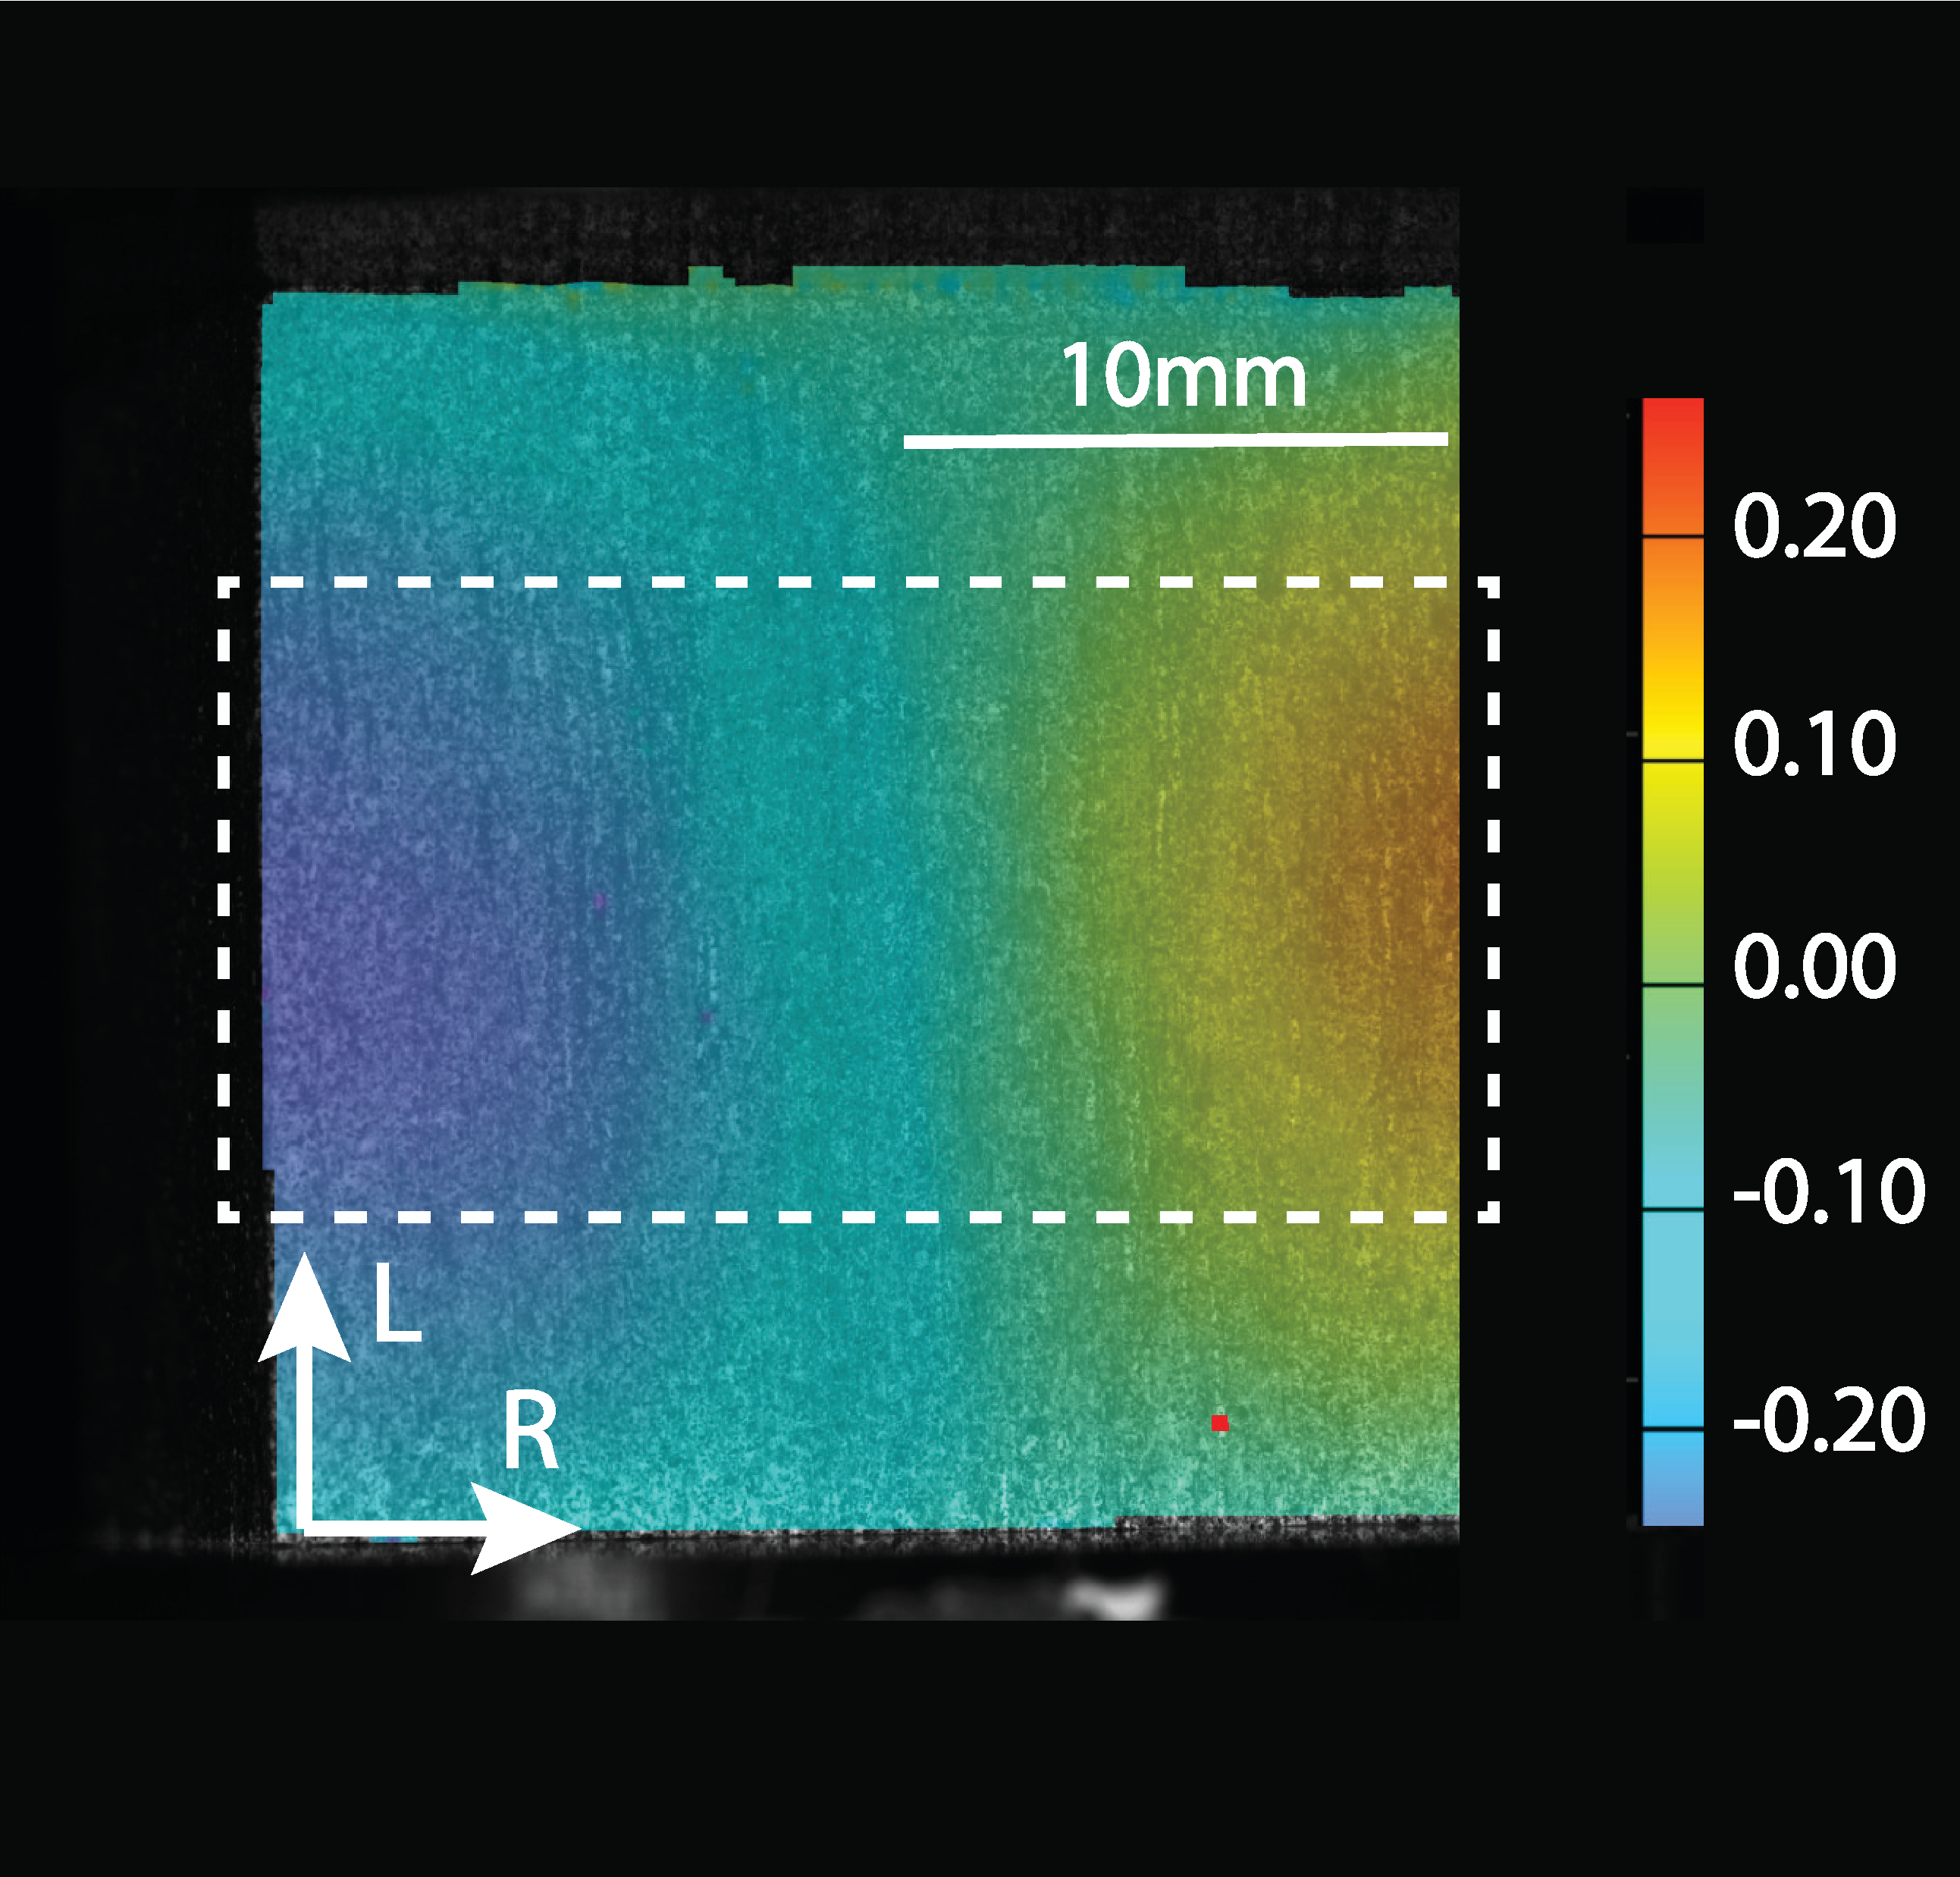
\includegraphics[width=\textwidth]{BarellingPaper-eps-converted-to.pdf}
        \caption{}
        \label{fig:experiment}
    \end{subfigure}
    \hfill
    \hspace*{-20px}
    \begin{subfigure}[b]{0.4\textwidth}
        \centering
        \pgfplotsset{every axis legend/.append style={
		at={(0.5,1.03)},
		anchor=east}}
		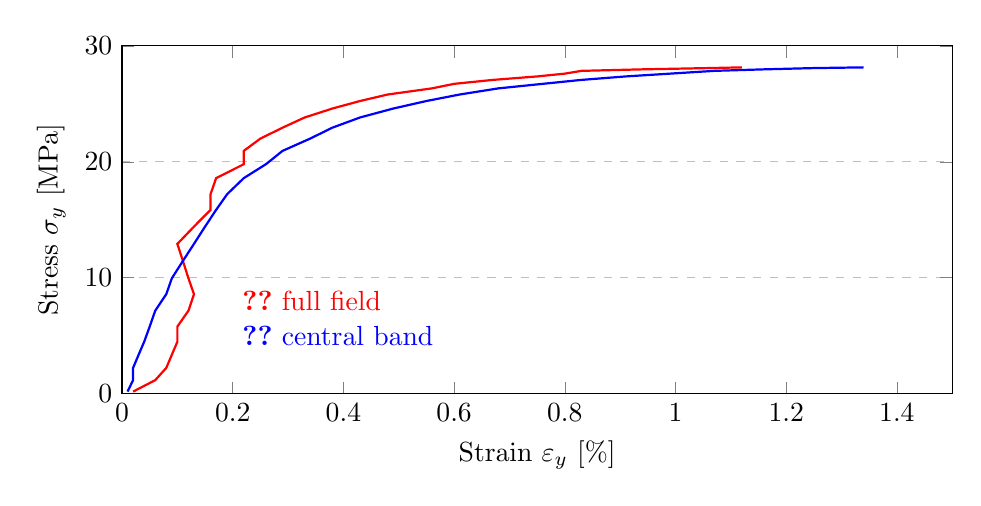
\begin{tikzpicture}
		\pgfplotstableread{
		stress	areaoi	totarea
		0.18	0.02	0.01
		1.17	0.06	0.02
		2.23	0.08	0.02
		3.36	0.09	0.03
		4.48	0.10	0.04
		5.79	0.10	0.05
		7.16	0.12	0.06
		8.59	0.13	0.08
		9.95	0.12	0.09
		11.45	0.11	0.11
		12.92	0.10	0.13
		14.41	0.13	0.15
		15.85	0.16	0.17
		17.21	0.16	0.19
		18.59	0.17	0.22
		19.79	0.22	0.26
		20.94	0.22	0.29
		22.00	0.25	0.34
		22.94	0.29	0.38
		23.82	0.33	0.43
		24.59	0.38	0.49
		25.24	0.43	0.55
		25.80	0.48	0.61
		26.33	0.56	0.68
		26.72	0.60	0.76
		27.06	0.67	0.83
		27.36	0.75	0.91
		27.60	0.80	0.99
		27.84	0.83	1.07
		27.97	0.94	1.16
		28.08	1.06	1.25
		28.14	1.12	1.34
		
		}\datatable
		
		
		
		
		\begin{axis}[no markers,
		name=plot0,height=6cm,width=\textwidth,
		    xlabel={Strain $\varepsilon_y$ [\%]},
		    ylabel={Stress $\sigma_y$ [MPa]},
		    xmin=0, xmax=1.5,
		    ymin=0, ymax=30,
		%     xtick={0,...,5},
		%    ytick={0,20,40,60,80},
		%     xticklabels={$0$,$0.2$,$0.4$,$0.6$,$0.8$, $1$}, 
		%     x tick label style={yshift=-1ex,
		%     rotate=45,anchor=east},
		    ymajorgrids=true,
		    grid style=dashed,
		]
		% \end{axis}    
		% \begin{axis}[legend pos=outer north east]
		 
		 
		    \addplot [thick, red] table[x=areaoi,y=stress] {\datatable};
		    \label{ex1}
		%     \addlegendentry{Total surface area}
		    \addplot [thick, blue] table[x=totarea,y=stress] {\datatable};
		    \label{ex2}
		%     \addlegendentry{Surface area of interest}
% 			\addplot [thin, red] coordinates {(0.0, 0.3) (0.28,28.0)};
% 			\addplot [thin, blue] coordinates {(0.05, 0.3) (0.25,28.0)};
\node at (axis cs:0.2,8) [anchor=west,red] {\ref{ex1} full field};
\node at (axis cs:0.2,5) [anchor=west,blue] {\ref{ex2} central band};
			
		
		\end{axis}
		
		\end{tikzpicture}		
        \caption{}
        \label{fig:explot}
    \end{subfigure}

\caption{(a) Vasa oak sample (b) Barrelling of an initially cubic shape.
(c) DSP image of Vasa oak sample during compressive testing including the
displacement field. (d) Experimental stress-strain curves for Vasa oak  sample
%, chosen surface area of interest(\ref{ex2}) and total surface area 
%(\ref{ex1})
.}
\label{fig:threegraphs}
\end{figure}












\begin{description}
\item{\textit{Numerical Model}}m
\end{description}





The finite element program COMSOL Multiphysics 4.4 \cite{Comsol} was used for
the numerical simulations.
A cube with unit dimensions was modelled with
3D solid elements.
The rig compliance was neglected since the platens were assumed to be rigid, leading to uniform normal displacement on the loaded surfaces.
The compressive loading was simulated as a downward vertical
displacement. The magnitude of this prescribed displacement was set to 0.01
which corresponds to an average compressive strain of  1\%.
A mesh refinement study showed that a $10\times10\times10$ mesh of quadratic
brick elements would provide sufficiently accurate results for the
purpose of this study.

\begin{figure}[h]
\centering
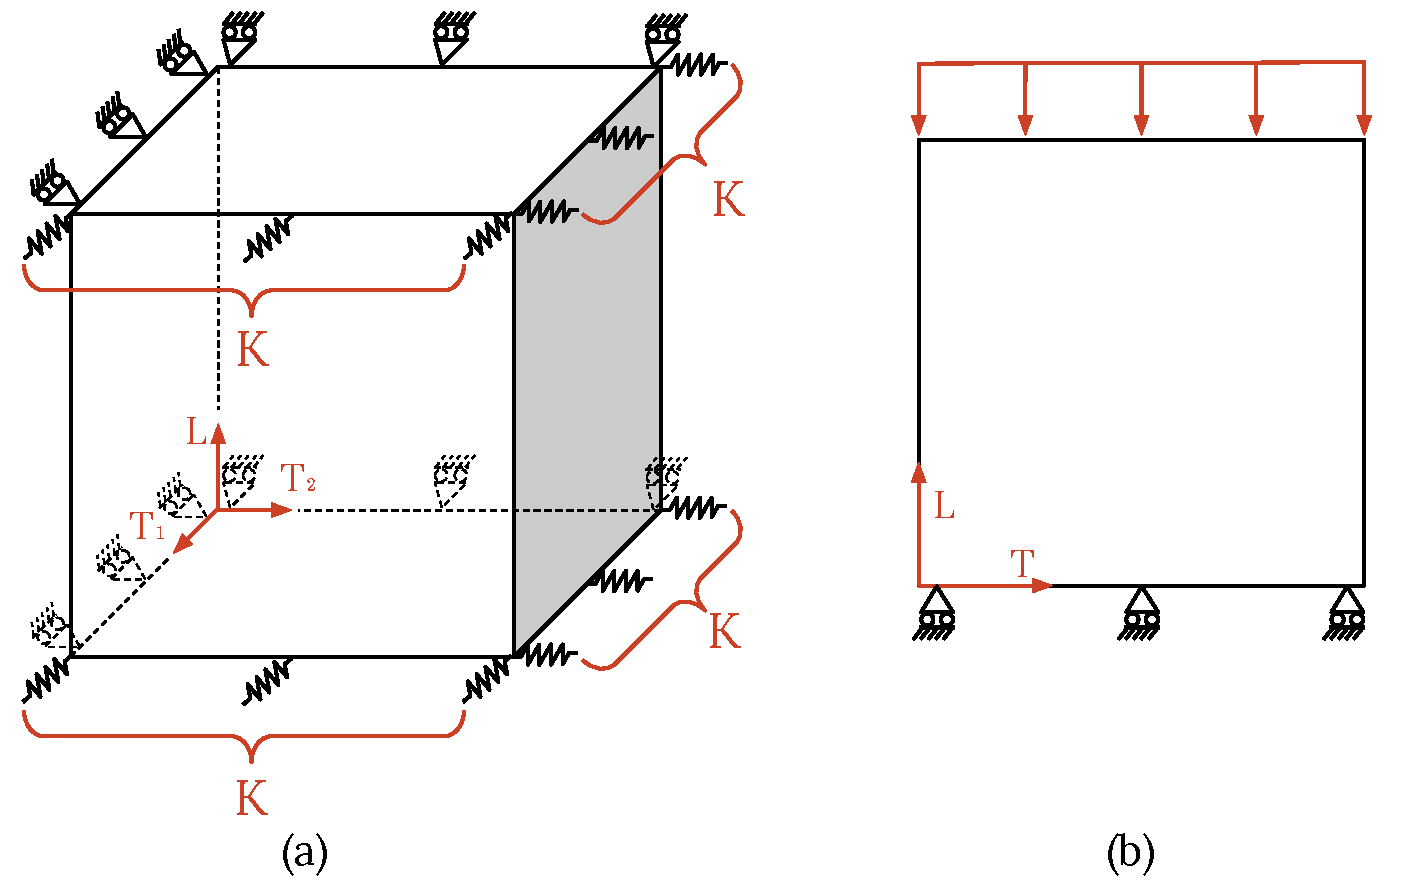
\includegraphics[width=8cm]{BarellingPaper.pdf}
\label{fig:Barrelling}
\caption{\label{fig:Barrelling} Model of cubic
sample used in the FEM simulation. 
(a) Horizontal boundary conditions and (b) vertical boundary conditions.}
\end{figure}

The main reason for the occurence of barrelling is the restraining friction
between the platens and the sample \cite{Narayanasamy198821, kulkarni1969}. To
simulate the effect of friction, we have introduced line springs with a spring
constant $K$ that is friction parameter in the model. Those springs are partially constrain lateral displacements
on the top and the bottom of the cube (Figure \ref{fig:Barrelling}).  
As a result, for $K=0$ the displacement of the corresponding
edges is unconstrained and for $K>0$ the edges are partially constrained up to
the case where the edges are completely constraint for $K=\infty$.

\begin{description}
\item{\textit{Material input parameters}}
\end{description}

Present work investigates isotropic, transversely isotropic and orthotropic
material behavior in combination with linear elasticity.
The material properties that were adopted are listed in
Table \ref{table:simulpar}. Two parameters $a$ and $b$ were introduced for a continuous transition between isotropy and transverse isotropy. 
The first one , $a$, is controlling the stiffness difference between the
longitudinal and transverse directions and the corresponding Poisson's ratio.
The second one, $b$, controls the independent shear modulus based on
observations of shear moduli for materials in Table \ref{table:nonlin}.
The remaining three Poisson's ratios were obtained from the symmetry
principle relations (symmetry of stiffness tensor\cite{hyer2009stress}). The
orthotropic material was simulated using input parameters obtained from the experiments \cite{vorobyevcharacterisation}.


\begin{description}
\item{\textit{Strain measuring methods}}
\end{description}


Three strain measuring cases were taken intro account in simulation. The first
case can be considered the same as taking the average dimensional changes of a
sample. In particular the average strain from the total surface area was
obtained and used as a value for obtaining axial stiffness $E_L$. In the
second case, $50\%$ of cube surface (Figure \ref{fig:experiment}) was
used to calculate the average strain corresponding to experimental measurement. 
Finally, in the third method the strain is measured between two points
in horizontal and two points in vertical direction in the center of the sample
as it is with the strain gauge based on ASTM-D143-94 standard
\cite{american2009standard}.

\begin{description}
\item{\textit{Experimental procedures}}
\end{description}

Finally we compare the results to an actual experiment on \textit{Vasa}
material.
An Instron universal testing machine with 100 kN load cell was used to carry out static tests. 
Special care was taken in order to manufacture almost exactly cubic samples. 
The size of the samples was  $25\times25\times25$ mm\textsuperscript{3}.  The
accuracy for parallelity between the opposite edges of the cube was 0.01 mm. 
Initial tests were conducted on dummy wood samples in order to find the approximate elastic loading range for all sample orientations.
Full-field displacements were observed with a DSP equipment GOM Aramis stereo system 5M.
The distance to the measured object was 300 mm. The surfaces of samples was spray
painted with speckles for better contrast. The applied force values were continuously recorded by the DSP system during testing, and stored together with the sampled images. The displacement rate was 0.5 mm per minute. 
The ambient conditions were $23\,^{\circ}{\rm C}$ and 51\% relative humidity.
All tests were performed without delay after the samples were removed from the conditioning storage container, so that the moisture content would essentially be the same as after conditioning. The measurement sampling frequency was 1 Hz. 
Every frame that was recorded by the DSP system was compared with the undeformed state in order to calculate the displacement and in-plane strain field. 
The total surface area of interest used in image analysis was a centred square
of 625 $mm\textsuperscript{2}$.
The chosen surface area of interest is marked by the dashed line in Figure
\ref{fig:experiment} and is about 350 $mm\textsuperscript{2}$ . The acquired
strain fields were smoothed by averaging of each data pixel with $3\times3$ surrounding pixels in order to avoid the
unwanted artifacts in the measured strain field.
The strains determined by DSP in the loading direction was plotted against the
applied stress, as exemplified in Figure \ref{fig:explot}. The choice of this
area is the subject of a later discussion in the present paper.
Poisson's ratios $\nu_{xy}$ for all corresponding orthotropic planes were
calculated as the negative ratio between the average transverse
$\varepsilon_{x}$ (passive) and normal $\varepsilon_{y}$ (compressive and
active) strains.


\begin{center}% note that \centering uses less vspace...
\begin{figure}[!ht]
\pgfplotsset{every axis legend/.append style={
		at={(0.5,1.03)},
		anchor=north}}

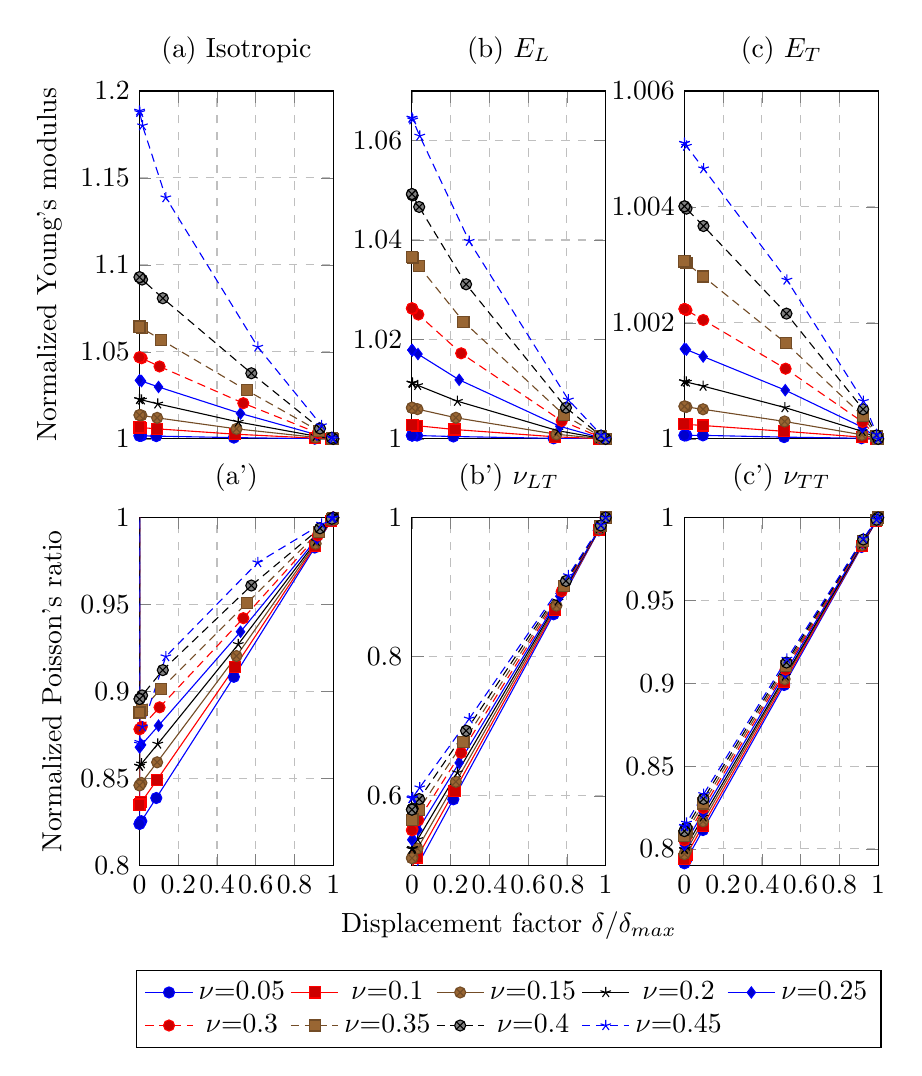
\begin{tikzpicture}[scale=1]

	\pgfplotstableread{
K	s1	0.05	s2	0.1	s3	0.15	s4	0.2	s5	0.25	s6	0.3	s7	0.35	s8	0.4	s9	0.45
1	1	1	1	1	1	1	1	1	1	1	1	1	1	1	1	1	1	1
2	1.00001	0.98959	1.00004	0.98983	1.00009	0.99013	1.00016	0.99049	1.00025	0.99091	1.00036	0.99141	1.00049	0.99201	1.00064	0.99273	1.00081	0.99366
3	1.0001	0.90485	1.00039	0.90684	1.00086	0.90934	1.00151	0.91237	1.00234	0.916	1.00335	0.92031	1.00455	0.92545	1.00598	0.93174	1.00768	0.94003
4	1.00071	0.48743	1.00269	0.49329	1.00574	0.50078	1.00972	0.51016	1.0146	0.52174	1.02051	0.53607	1.02786	0.55404	1.03771	0.57742	1.05282	0.61085
5	1.00157	0.08684	1.00577	0.08872	1.01207	0.09119	1.02012	0.09437	1.02983	0.09844	1.04161	0.1037	1.05701	0.11069	1.08084	0.12049	1.13869	0.1361
6	1.00176	0.00942	1.00647	0.00964	1.01348	0.00994	1.02243	0.01031	1.03322	0.0108	1.04635	0.01144	1.0637	0.0123	1.09157	0.01353	1.18008	0.01554
7	1.00178	0.00095009	1.00654	0.00097274	1.01364	0.001	1.02269	0.00104	1.0336	0.00109	1.04688	0.00116	1.06446	0.00124	1.09282	0.00137	1.18771	0.00158
8	1.00179	9.50903E-05	1.00655	9.73593E-05	1.01366	0.000100348	1.02272	0.000104217	1.03364	0.000109217	1.04693	0.000115754	1.06454	0.00012456	1.09295	0.000137156	1.18856	0.000157846

}\datatable

\pgfplotstableread{
K	s1	0.05	s2	0.1	s3	0.15	s4	0.2	s5	0.25	s6	0.3	s7	0.35	s8	0.4	s9	0.45
0	1	1	1	1	1	1	1	1	1	1	1	1	1	1	1	1	1	1
0.001	1.00001	0.96454	1.00004	0.96576	1.00009	0.96707	1.00016	0.96846	1.00025	0.96993	1.00036	0.97149	1.00049	0.97314	1.00064	0.97488	1.00081	0.97672
0.01	1.0001	0.73119	1.00041	0.73827	1.00092	0.74597	1.00163	0.75431	1.00252	0.76334	1.0036	0.77311	1.00485	0.78368	1.00627	0.79513	1.00786	0.80754
0.1	1.00047	0.21384	1.00188	0.22002	1.00424	0.227	1.00757	0.23491	1.01188	0.2439	1.01721	0.25418	1.02359	0.26598	1.0311	0.27966	1.03978	0.29565
1	1.00066	0.02648	1.00264	0.02744	1.00598	0.02853	1.01076	0.02979	1.01706	0.03126	1.02501	0.03296	1.03479	0.03498	1.04666	0.03739	1.06095	0.04031
10	1.00068	0.00271	1.00274	0.00281	1.00623	0.00293	1.01121	0.00306	1.0178	0.00322	1.02614	0.0034	1.03644	0.00361	1.04899	0.00387	1.06421	0.00418
100	1.00068	0.000271937	1.00275	0.000282014	1.00625	0.0002936	1.01126	0.000306985	1.01787	0.000322546	1.02625	0.000340787	1.03661	0.000362391	1.04924	0.000388305	1.06455	0.000419892
1000	1.00068	2.72003E-05	1.00275	2.82085E-05	1.00625	2.93678E-05	1.01126	3.07069E-05	1.01788	0.000032264	1.02627	3.40892E-05	1.03663	3.62509E-05	1.04926	3.88442E-05	1.06458	4.20052E-05


}\datatableA

\pgfplotstableread{
K	s1	0.05	s2	0.1	s3	0.15	s4	0.2	s5	0.25	s6	0.3	s7	0.35	s8	0.4	s9	0.45
0	1	1	1	1	1	1	1	1	1	1	1	1	1	1	1	1	1	1
0.001	1	0.99079	1	0.99096	1.00001	0.99114	1.00002	0.99132	1.00002	0.99151	1.00004	0.9917	1.00005	0.9919	1.00006	0.9921	1.00008	0.9923
0.01	1.00001	0.91454	1.00003	0.91559	1.00007	0.91669	1.00013	0.91784	1.0002	0.91904	1.00029	0.92028	1.00039	0.92157	1.00051	0.92291	1.00065	0.9243
0.1	1.00003	0.51477	1.00013	0.51597	1.0003	0.51733	1.00054	0.51887	1.00084	0.52059	1.00121	0.52248	1.00165	0.52456	1.00216	0.52682	1.00274	0.52927
1	1.00006	0.0957	1.00023	0.09591	1.00051	0.09618	1.00091	0.09651	1.00142	0.0969	1.00205	0.09735	1.0028	0.09787	1.00367	0.09846	1.00466	0.09912
10	1.00006	0.01047	1.00025	0.01049	1.00055	0.01052	1.00098	0.01056	1.00154	0.0106	1.00222	0.01065	1.00303	0.01071	1.00397	0.01078	1.00505	0.01086
100	1.00006	0.00106	1.00025	0.00106	1.00056	0.00106	1.00099	0.00107	1.00155	0.00107	1.00224	0.00108	1.00306	0.00108	1.00401	0.00109	1.0051	0.0011
1000	1.00006	0.000105788	1.00025	0.000106007	1.00056	0.000106301	1.00099	0.00010667	1.00155	0.000107116	1.00224	0.000107641	1.00306	0.000108246	1.00401	0.000108934	1.0051	0.000109708



}\datatableB

\pgfplotstableread{
K	p1	0.05	p2	0.1	p3	0.15	p4	0.2	p5	0.25	p6	0.3	p7	0.35	p8	0.4	p9	0.45
1	1	1	1	1	1	1	1	1	1	1	1	1	1	1	1	1	1	1
2	0.99811	0.98959	0.99822	0.98983	0.99836	0.99013	0.99851	0.99049	0.99869	0.99091	0.99889	0.99141	0.99911	0.99201	0.99935	0.99273	0.99962	0.99366
3	0.98278	0.90485	0.98381	0.90684	0.98503	0.90934	0.98641	0.91237	0.98798	0.916	0.98973	0.92031	0.99168	0.92545	0.99387	0.93174	0.99633	0.94003
4	0.90847	0.48743	0.91417	0.49329	0.92042	0.50078	0.92716	0.51016	0.93439	0.52174	0.94218	0.53607	0.95081	0.55404	0.96094	0.57742	0.97419	0.61085
5	0.8388	0.08684	0.84892	0.08872	0.85932	0.09119	0.86987	0.09437	0.88042	0.09844	0.89092	0.1037	0.90149	0.11069	0.91232	0.12049	0.92012	0.1361
6	0.82548	0.00942	0.8364	0.00964	0.84747	0.00994	0.85851	0.01031	0.86932	0.0108	0.87971	0.01144	0.88953	0.0123	0.89776	0.01353	0.87979	0.01554
7	0.82403	0.00095009	0.83503	0.00097274	0.84617	0.001	0.85725	0.00104	0.86807	0.00109	0.87843	0.00116	0.8881	0.00124	0.89587	0.00137	0.87093	0.00158
8	0.82388	9.50903E-05	0.83489	9.73593E-05	0.84603	0.000100348	0.85713	0.000104217	0.86795	0.000109217	0.8783	0.000115754	0.88795	0.00012456	0.89568	0.000137156	0.86991	0.000157846
9	1.00179	9.50903E-05	1.00655	9.73593E-05	1.01366	0.000100348	1.02272	0.000104217	1.03364	0.000109217	1.04693	0.000115754	1.06454	0.00012456	1.09295	0.000137156	1.18856	0.000157846


}\datatableC

\pgfplotstableread{
K	p1	0.05	p2	0.1	p3	0.15	p4	0.2	p5	0.25	p6	0.3	p7	0.35	p8	0.4	p9	0.45
0	1	1	1	1	1	1	1	1	1	1	1	1	1	1	1	1	1	1
0.001	0.98163	0.96454	0.98255	0.96576	0.9835	0.96707	0.98446	0.96846	0.98546	0.96993	0.98647	0.97149	0.98752	0.97314	0.98859	0.97488	0.98969	0.97672
0.01	0.86103	0.73119	0.86719	0.73827	0.87356	0.74597	0.88015	0.75431	0.88696	0.76334	0.89402	0.77311	0.90133	0.78368	0.90892	0.79513	0.9168	0.80754
0.1	0.59508	0.21384	0.60748	0.22002	0.62028	0.227	0.63358	0.23491	0.64744	0.2439	0.66198	0.25418	0.67731	0.26598	0.69357	0.27966	0.7109	0.29565
1	0.49897	0.02648	0.51154	0.02744	0.52436	0.02853	0.5375	0.02979	0.55107	0.03126	0.56517	0.03296	0.57992	0.03498	0.59544	0.03739	0.61191	0.04031
10	0.48675	0.00271	0.49923	0.00281	0.51193	0.00293	0.52492	0.00306	0.53829	0.00322	0.55215	0.0034	0.5666	0.00361	0.58178	0.00387	0.59782	0.00418
100	0.48549	2.72E-04	0.49796	2.82E-04	0.51065	2.94E-04	0.52362	3.07E-04	0.53697	3.23E-04	0.55081	3.41E-04	0.56523	3.62E-04	0.58036	3.88E-04	0.59635	4.20E-04
1000	0.48536	2.72E-05	0.49784	2.82E-05	0.51052	2.94E-05	0.52349	3.07E-05	0.53684	3.23E-05	0.55067	3.41E-05	0.56509	3.63E-05	0.58022	3.88E-05	0.5962	4.20E-05



}\datatableD

\pgfplotstableread{
K	p1	0.05	p2	0.1	p3	0.15	p4	0.2	p5	0.25	p6	0.3	p7	0.35	p8	0.4	p9	0.45
0	1	1	1	1	1	1	1	1	1	1	1	1	1	1	1	1	1	1
0.001	0.9981	0.99079	0.99818	0.99096	0.99826	0.99114	0.99835	0.99151	0.99844	0.99151	0.99853	0.9917	0.99862	0.9919	0.99871	0.9921	0.9988	0.9923
0.01	0.98229	0.91454	0.98288	0.91559	0.98348	0.91669	0.98409	0.91904	0.98473	0.91904	0.98539	0.92028	0.98606	0.92157	0.98675	0.92291	0.98746	0.9243
0.1	0.89895	0.51477	0.90071	0.51597	0.90253	0.51733	0.90441	0.52059	0.90634	0.52059	0.90833	0.52248	0.91038	0.52456	0.9125	0.52682	0.91467	0.52927
1	0.81141	0.0957	0.81404	0.09591	0.81668	0.09618	0.81934	0.0969	0.82202	0.0969	0.82472	0.09735	0.82745	0.09787	0.83021	0.09846	0.833	0.09912
10	0.79351	0.01047	0.79628	0.01049	0.79903	0.01052	0.80179	0.0106	0.80455	0.0106	0.80732	0.01065	0.81011	0.01071	0.8129	0.01078	0.81571	0.01086
100	0.79153	0.00106	0.7943	0.00106	0.79707	0.00106	0.79984	0.00107	0.8026	0.00107	0.80538	0.00108	0.80816	0.00108	0.81095	0.00109	0.81376	0.0011
1000	0.79133	0.000105788	0.7941	0.000106007	0.79687	0.000106301	0.79964	0.000107116	0.8024	0.000107116	0.80518	0.000107641	0.80796	0.000108246	0.81075	0.000108934	0.81356	0.000109708


}\datatableE



\begin{axis}[
name=plot0,height=6cm,width=\textwidth/3,
    title={(a) Isotropic},
%    xlabel={Temperature [\textcelsius]},
    ylabel={Normalized Young's modulus},
    xmin=0, xmax=1,
    ymin=1, ymax=1.2,
%     xtick={1,...,9},
%    ytick={0,20,40,60,80},
    xticklabels={}, 
    ymajorgrids=true,
    xmajorgrids=true,
    grid style=dashed,
]
% \end{axis}    
% \begin{axis}[legend pos=outer north east]
 
 
    \addplot table[y=s1,x=0.05] {\datatable};
%     \addlegendentry{$\nu$=0.05}
    \addplot table[y=s2,x=0.1] {\datatable};
%     \addlegendentry{$\nu$=0.1}
    \addplot table[y=s3,x=0.15] {\datatable};
%     \addlegendentry{$\nu$=0.15}
    \addplot table[y=s4,x=0.2] {\datatable};
%     \addlegendentry{$\nu$=0.2}
    \addplot table[y=s5,x=0.25] {\datatable};
%     \addlegendentry{$\nu$=0.25}
    \addplot table[y=s6,x=0.3] {\datatable};
%     \addlegendentry{$\nu$=0.3}
    \addplot table[y=s7,x=0.35] {\datatable};
%     \addlegendentry{$\nu$=0.35}
    \addplot table[y=s8,x=0.4] {\datatable};
%     \addlegendentry{$\nu$=0.4}
    \addplot table[y=s9,x=0.45] {\datatable};
%     \addlegendentry{$\nu$=0.45}

% \draw	(70,160) node{{Isotropic}};
\end{axis}

\begin{axis}[
name=plot1,at={($(plot0.east)+(1cm,0)$)},anchor=west,
height=6cm,width=\textwidth/3, title={(b) $E_L$},
%    xlabel={Temperature [\textcelsius]},
%    ylabel={Measured stiffness [Pa]},
    xmin=0, xmax=1,
    ymin=1, ymax=1.07,
    yticklabel style={/pgf/number format/fixed,
                  /pgf/number format/precision=3},
%     xtick={1,...,9},
%    ytick={0,20,40,60,80},
%     xticklabels={$0$,$0.001$,$0.01$,$0.1$,$1$, $10$, $100$,
%     $1000$, $\infty$}, 
    xticklabels={}, 
    ymajorgrids=true,
    xmajorgrids=true,
    grid style=dashed,
]

    \addplot table[y=s1,x=0.05] {\datatableA};
%     \addlegendentry{$\nu$=0.05}
    \addplot table[y=s2,x=0.1] {\datatableA};
%     \addlegendentry{$\nu$=0.1}
    \addplot table[y=s3,x=0.15] {\datatableA};
%     \addlegendentry{$\nu$=0.15}
    \addplot table[y=s4,x=0.2] {\datatableA};
%     \addlegendentry{$\nu$=0.2}
    \addplot table[y=s5,x=0.25] {\datatableA};
%     \addlegendentry{$\nu$=0.25}
    \addplot table[y=s6,x=0.3] {\datatableA};
%     \addlegendentry{$\nu$=0.3}
    \addplot table[y=s7,x=0.35] {\datatableA};
%     \addlegendentry{$\nu$=0.35}
    \addplot table[y=s8,x=0.4] {\datatableA};
%     \addlegendentry{$\nu$=0.4}
    \addplot table[y=s9,x=0.45] {\datatableA};
%     \addlegendentry{$\nu$=0.45}


\end{axis}

\begin{axis}[
	name=plot2,at={($(plot1.east)+(1cm,0)$)},anchor=west, height=6cm,width=\textwidth/3,
    title={(c) $E_T$},
%    xlabel={Temperature [\textcelsius]},
%    ylabel={Measured stiffness [Pa]},
    xmin=0, xmax=1,
    ymin=1, ymax=1.006,
    yticklabel style={/pgf/number format/fixed,
                  /pgf/number format/precision=3},
%     xtick={1,...,9},
%    ytick={0,20,40,60,80},
    xticklabels={}, 
    ymajorgrids=true,
    xmajorgrids=true,
    grid style=dashed,
    bar shift=0pt
]

    \addplot table[y=s1,x=0.05] {\datatableB};
%     \addlegendentry{$\nu$=0.05}
    \addplot table[y=s2,x=0.1] {\datatableB};
%     \addlegendentry{$\nu$=0.1}
    \addplot table[y=s3,x=0.15] {\datatableB};
%     \addlegendentry{$\nu$=0.15}
    \addplot table[y=s4,x=0.2] {\datatableB};
%     \addlegendentry{$\nu$=0.2}
    \addplot table[y=s5,x=0.25] {\datatableB};
%     \addlegendentry{$\nu$=0.25}
    \addplot table[y=s6,x=0.3] {\datatableB};
%     \addlegendentry{$\nu$=0.3}
    \addplot table[y=s7,x=0.35] {\datatableB};
%     \addlegendentry{$\nu$=0.35}
    \addplot table[y=s8,x=0.4] {\datatableB};
%     \addlegendentry{$\nu$=0.4}
    \addplot table[y=s9,x=0.45] {\datatableB};
%     \addlegendentry{$\nu$=0.45}


\end{axis}

\begin{axis}[name=plot3,at={($(plot0.south)-(0,1cm)$)},anchor=north,
height=6cm,width=\textwidth/3, title={(a')},
%    xlabel={Temperature [\textcelsius]},
    ylabel={Normalized Poisson's ratio},
    xmin=0, xmax=1,
    ymin=0.8, ymax=1,
%     xtick={1,...,9},
%    ytick={0,20,40,60,80},
%     xticklabels={$0$,$0.001$,$0.01$,$0.1$,$1$, $10$, $100$,
%     $1000$, $\infty$}, 
%     x tick label style={yshift=-1ex,
%     rotate=45,anchor=east},
    ymajorgrids=true,
    xmajorgrids=true,
    grid style=dashed,
]
% \end{axis}    
% \begin{axis}[legend pos=outer north east]
 
 
    \addplot table[y=p1,x=0.05] {\datatableC};
%     \addlegendentry{$\nu$=0.05}
    \addplot table[y=p2,x=0.1] {\datatableC};
%     \addlegendentry{$\nu$=0.1}
    \addplot table[y=p3,x=0.15] {\datatableC};
%     \addlegendentry{$\nu$=0.15}
    \addplot table[y=p4,x=0.2] {\datatableC};
%     \addlegendentry{$\nu$=0.2}
    \addplot table[y=p5,x=0.25] {\datatableC};
%     \addlegendentry{$\nu$=0.25}
    \addplot table[y=p6,x=0.3] {\datatableC};
%     \addlegendentry{$\nu$=0.3}
    \addplot table[y=p7,x=0.35] {\datatableC};
%     \addlegendentry{$\nu$=0.35}
    \addplot table[y=p8,x=0.4] {\datatableC};
%     \addlegendentry{$\nu$=0.4}
    \addplot table[y=p9,x=0.45] {\datatableC};
%     \addlegendentry{$\nu$=0.45}
\end{axis}

\begin{axis}[legend style={at={(0.5,-0.3)}, legend columns=5, anchor=north},
	name=plot4,at={($(plot1.south)-(0,1cm)$)},anchor=north, height=6cm,width=\textwidth/3,
    title={(b') $\nu_{LT}$},
    xlabel={Displacement factor $\delta/\delta_{max}$},
%    ylabel={Measured stiffness [Pa]},
    xmin=0, xmax=1,
    ymin=0.5, ymax=1,
    yticklabel style={/pgf/number format/fixed,
                  /pgf/number format/precision=3},
%     xtick={1,...,9},
%    ytick={0,20,40,60,80},
%     xticklabels={$0$,$0.001$,$0.01$,$0.1$,$1$, $10$, $100$,
%     $1000$, $\infty$}, 
%     x tick label style={yshift=-1ex,
%         rotate=45,anchor=east},
    ymajorgrids=true,
    xmajorgrids=true,
    grid style=dashed,
    bar shift=0pt
]

    \addplot table[y=p1,x=0.05] {\datatableD};
     \addlegendentry{$\nu$=0.05}
    \addplot table[y=p2,x=0.1] {\datatableD};
     \addlegendentry{$\nu$=0.1}
    \addplot table[y=p3,x=0.15] {\datatableD};
     \addlegendentry{$\nu$=0.15}
    \addplot table[y=p4,x=0.2] {\datatableD};
     \addlegendentry{$\nu$=0.2}
    \addplot table[y=p5,x=0.25] {\datatableD};
     \addlegendentry{$\nu$=0.25}
    \addplot table[y=p6,x=0.3] {\datatableD};
     \addlegendentry{$\nu$=0.3}
    \addplot table[y=p7,x=0.35] {\datatableD};
     \addlegendentry{$\nu$=0.35}
    \addplot table[y=p8,x=0.4] {\datatableD};
     \addlegendentry{$\nu$=0.4}
    \addplot table[y=p9,x=0.45] {\datatableD};
     \addlegendentry{$\nu$=0.45}

\end{axis}


\begin{axis}[
	name=plot5,at={($(plot2.south)-(0,1cm)$)},anchor=north, height=6cm,width=\textwidth/3,
    title={(c') $\nu_{TT}$},
%    xlabel={Temperature [\textcelsius]},
%    ylabel={Measured stiffness [Pa]},
    xmin=0, xmax=1,
    ymin=0.79, ymax=1.,
    yticklabel style={/pgf/number format/fixed,
                  /pgf/number format/precision=3},
%     xtick={1,...,9},
%    ytick={0,20,40,60,80},
%     xticklabels={$0$,$0.001$,$0.01$,$0.1$,$1$, $10$, $100$,
%     $1000$, $\infty$}, 
%         x tick label style={yshift=-1ex,
%         rotate=45,anchor=east		},
    ymajorgrids=true,
    xmajorgrids=true,
    grid style=dashed,
    bar shift=0pt
]

    \addplot table[y=p1,x=0.05] {\datatableE};
%     \addlegendentry{$\nu$=0.05}
    \addplot table[y=p2,x=0.1] {\datatableE};
%     \addlegendentry{$\nu$=0.1}
    \addplot table[y=p3,x=0.15] {\datatableE};
%     \addlegendentry{$\nu$=0.15}
    \addplot table[y=p4,x=0.2] {\datatableE};
%     \addlegendentry{$\nu$=0.2}
    \addplot table[y=p5,x=0.25] {\datatableE};
%     \addlegendentry{$\nu$=0.25}
    \addplot table[y=p6,x=0.3] {\datatableE};
%     \addlegendentry{$\nu$=0.3}
    \addplot table[y=p7,x=0.35] {\datatableE};
%     \addlegendentry{$\nu$=0.35}
    \addplot table[y=p8,x=0.4] {\datatableE};
%     \addlegendentry{$\nu$=0.4}
    \addplot table[y=p9,x=0.45] {\datatableE};
%     \addlegendentry{$\nu$=0.45}

\end{axis}


\end{tikzpicture}


\captionsetup{justification=centering}
\caption{a) Simulated and normalized Young's moduli values of material with
different given Poisson's ratio ($\nu$) values for isotropic material ($a=1$),
b) $E_L$, and c) $E_T$ for transversely isotropic material ($a=10$; $b=2$).
a') Simulated Poisson's ratio error values of material with different given
Poisson's ratio ($\nu$) values for isotropic material, b')
$\nu_{LT},$ and c') $\nu_{TL}$ for transversely isotropic material.}


\label{fig:isovstriso}
\end{figure}

\end{center}

% 
% \begin{center}% note that \centering uses less vspace...
% \begin{figure}[!ht]
% \pgfplotsset{every axis legend/.append style={
% 		at={(0.5,1.03)},
% 		anchor=north}}
% 
% \begin{tikzpicture}[scale=1]
% 
% 	\pgfplotstableread{
% 	K	0.05	0.1	0.15	0.2	0.25	0.3	0.35	0.4	0.45
% 1	1	1	1	1	1	1	1	1	1
% 2	1.00001	1.00002	1.00004	1.00008	1.00013	1.00018	1.00025	1.00033	1.00042
% 3	1.00005	1.00019	1.00043	1.00076	1.00121	1.00174	1.00241	1.00319	1.00412
% 4	1.00032	1.00127	1.00283	1.00505	1.00802	1.01194	1.01722	1.02472	1.03666
% 5	1.00075	1.00292	1.00645	1.0115	1.01853	1.02879	1.04539	1.07813	1.18128
% 6	1.00087	1.00335	1.0074	1.01319	1.02137	1.03365	1.0547	1.10164	1.34588
% 7	1.00089	1.00341	1.00751	1.01339	1.0217	1.03423	1.05589	1.10502	1.39391
% 8	1.00089	1.00341	1.00752	1.0134	1.02174	1.03429	1.05602	1.10538	1.39995
% 9	1.00089	1.00341	1.00752	1.01341	1.02174	1.0343	1.05603	1.10542	1.40064
% }\datatable
% 
% \pgfplotstableread{
% K	0.05	0.1	0.15	0.2	0.25	0.3	0.35	0.4	0.45
% 1	1	1	1	1	1	1	1	1	1
% 2	1	1.00001	1.00002	1.00003	1.00004	1.00005	1.00006	1.00006	1.00005
% 3	1.00002	1.00008	1.00016	1.00024	1.00033	1.0004	1.00045	1.00046	1.00043
% 4	1.00006	1.00023	1.00048	1.00077	1.00107	1.00135	1.00156	1.00166	1.0016
% 5	1.00008	1.00029	1.00061	1.00098	1.00138	1.00176	1.00206	1.00222	1.00219
% 6	1.00008	1.0003	1.00062	1.00101	1.00142	1.00181	1.00213	1.0023	1.00226
% 7	1.00008	1.0003	1.00062	1.00101	1.00143	1.00182	1.00213	1.00231	1.00227
% 8	1.00008	1.0003	1.00062	1.00101	1.00143	1.00182	1.00213	1.00231	1.00227
% 9	1.00008	1.0003	1.00062	1.00101	1.00143	1.00182	1.00213	1.00231	1.00227
% 
% }\datatableA
% 
% \pgfplotstableread{
% K	0.05	0.1	0.15	0.2	0.25	0.3	0.35	0.4	0.45
% 1	1	1	1	1	1	1	1	1	1
% 2	1	1.0001	1.0002	1.0004	1.0007	1.001	1.0014	1.002	1.0026
% 3	1.0002	1.0007	1.0016	1.003	1.0048	1.0072	1.0101	1.0138	1.0183
% 4	1.0004	1.0017	1.0038	1.0071	1.0116	1.0174	1.0249	1.0344	1.0462
% 5	1.0005	1.0019	1.0044	1.0081	1.0132	1.0198	1.0283	1.0389	1.0523
% 6	1.0005	1.0019	1.0045	1.0082	1.0133	1.0199	1.0284	1.0391	1.0524
% 7	1.0005	1.0019	1.0045	1.0082	1.0133	1.0199	1.0284	1.0391	1.0524
% 8	1.0005	1.0019	1.0045	1.0082	1.0133	1.0199	1.0284	1.0391	1.0524
% 9	1.0005	1.0019	1.0045	1.0082	1.0133	1.0199	1.0284	1.0391	1.0524
% 
% 
% }\datatableB
% 
% \pgfplotstableread{
% 	K	0.05	0.1	0.15	0.2	0.25	0.3	0.35	0.4	0.45
% 1	1	1	1	1	1	1	1	1	1
% 2	0.9994	0.9995	0.999666667	0.99975	0.99984	0.999933333	1.000028571	1.0001	1.000177778
% 3	0.9948	0.9958	0.996733333	0.9977	0.99856	0.9994	1.0002	1.0009	1.001577778
% 4	0.972	0.9771	0.982133333	0.9871	0.99188	0.996566667	1.001114286	1.005525	1.009977778
% 5	0.9502	0.9591	0.967733333	0.9764	0.98496	0.9935	1.002085714	1.010875	1.020644444
% 6	0.946	0.9556	0.965	0.9743	0.98356	0.9928	1.002171429	1.011825	1.022711111
% 7	0.9456	0.9552	0.964666667	0.97405	0.9834	0.992733333	1.002171429	1.011925	1.022911111
% 8	0.9456	0.9552	0.964666667	0.97405	0.98336	0.992733333	1.002171429	1.011925	1.022933333
% 9	0.9456	0.9552	0.964666667	0.97405	0.98336	0.992733333	1.002171429	1.011925	1.022933333
% 
% }\datatableC
% 
% \pgfplotstableread{
% K	0.05	0.1	0.15	0.2	0.25	0.3	0.35	0.4	0.45
% 1	1	1	1	1	1	1	1	1	1
% 2	0.987	0.988	0.989	0.98995	0.99084	0.991766667	0.992657143	0.9935	0.994333333
% 3	0.9012	0.9079	0.914533333	0.9211	0.92756	0.934	0.940342857	0.9466	0.9528
% 4	0.7104	0.7239	0.737466667	0.7511	0.76496	0.778966667	0.793228571	0.807825	0.822866667
% 5	0.641	0.6551	0.669066667	0.6831	0.69724	0.711533333	0.726085714	0.740925	0.7562
% 6	0.6324	0.6463	0.660266667	0.67425	0.68836	0.702566667	0.717	0.7317	0.746822222
% 7	0.6314	0.6454	0.659333333	0.67335	0.68744	0.701633333	0.716057143	0.73075	0.745844444
% 8	0.6314	0.6453	0.659266667	0.67325	0.68736	0.701566667	0.715971429	0.730675	0.745755556
% 9	0.6314	0.6453	0.659266667	0.67325	0.68736	0.701566667	0.715971429	0.730675	0.745755556
% 
% 
% 
% }\datatableD
% 
% \pgfplotstableread{
% K	0.05	0.1	0.15	0.2	0.25	0.3	0.35	0.4	0.45
% 1	1	1	1	1	1	1	1	1	1
% 2	0.9902	0.99	0.9898	0.9897	0.98964	0.9896	0.989628571	0.989725	0.989888889
% 3	0.9328	0.9315	0.930266667	0.9292	0.92832	0.927733333	0.927428571	0.927475	0.927955556
% 4	0.84	0.8365	0.833266667	0.83015	0.82724	0.8246	0.822285714	0.820325	0.8188
% 5	0.815	0.8118	0.8088	0.80595	0.80328	0.800933333	0.798828571	0.797075	0.795733333
% 6	0.8122	0.8094	0.8066	0.80405	0.80172	0.799666667	0.797885714	0.7965	0.795533333
% 7	0.812	0.8091	0.8064	0.8039	0.80164	0.7996	0.797885714	0.79655	0.795644444
% 8	0.812	0.8091	0.8064	0.8039	0.8016	0.7996	0.797885714	0.79655	0.795666667
% 9	0.812	0.8091	0.8064	0.8039	0.8016	0.7996	0.797885714	0.79655	0.795666667
% 
% }\datatableE
% 
% 
% 
% \begin{axis}[
% name=plot0,height=6cm,width=5cm,
%     title={a)},
% %    xlabel={Temperature [\textcelsius]},
%     ylabel={Normalized Young's modulus},
%     xmin=1, xmax=9,
%     ymin=0.99, ymax=1.5,
%     xtick={1,...,9},
% %    ytick={0,20,40,60,80},
%     xticklabels={}, 
%     ymajorgrids=true,
%     xmajorgrids=true,
%     grid style=dashed,
% ]
% % \end{axis}    
% % \begin{axis}[legend pos=outer north east]
%  
%  
%     \addplot table[x=K,y=0.05] {\datatable};
% %     \addlegendentry{$\nu$=0.05}
%     \addplot table[x=K,y=0.1] {\datatable};
% %     \addlegendentry{$\nu$=0.1}
%     \addplot table[x=K,y=0.15] {\datatable};
% %     \addlegendentry{$\nu$=0.15}
%     \addplot table[x=K,y=0.2] {\datatable};
% %     \addlegendentry{$\nu$=0.2}
%     \addplot table[x=K,y=0.25] {\datatable};
% %     \addlegendentry{$\nu$=0.25}
%     \addplot table[x=K,y=0.3] {\datatable};
% %     \addlegendentry{$\nu$=0.3}
%     \addplot table[x=K,y=0.35] {\datatable};
% %     \addlegendentry{$\nu$=0.35}
%     \addplot table[x=K,y=0.4] {\datatable};
% %     \addlegendentry{$\nu$=0.4}
%     \addplot table[x=K,y=0.45] {\datatable};
% %     \addlegendentry{$\nu$=0.45}
% \end{axis}
% 
% \begin{axis}[
% name=plot1,at={($(plot0.east)+(1cm,0)$)},anchor=west,
% height=6cm,width=5cm, title={b)},
% %    xlabel={Temperature [\textcelsius]},
% %    ylabel={Measured stiffness [Pa]},
%     xmin=1, xmax=9,
%     ymin=1, ymax=1.003,
%     yticklabel style={/pgf/number format/fixed,
%                   /pgf/number format/precision=3},
%     xtick={1,...,9},
% %    ytick={0,20,40,60,80},
% %     xticklabels={$0$,$0.001$,$0.01$,$0.1$,$1$, $10$, $100$,
% %     $1000$, $\infty$}, 
%     xticklabels={}, 
%     ymajorgrids=true,
%     xmajorgrids=true,
%     grid style=dashed,
%     bar shift=0pt
% ]
% 
% 	\addplot table[x=K,y=0.05] {\datatableA};
% %      \addlegendentry{$\nu$=0.05}
%     \addplot table[x=K,y=0.1] {\datatableA};
% %      \addlegendentry{$\nu$=0.1}
%     \addplot table[x=K,y=0.15] {\datatableA};
% %     \addlegendentry{$\nu$=0.15}
%     \addplot table[x=K,y=0.2] {\datatableA};
% %      \addlegendentry{$\nu$=0.2}
%     \addplot table[x=K,y=0.25] {\datatableA};
% %      \addlegendentry{$\nu$=0.25}
%     \addplot table[x=K,y=0.3] {\datatableA};
% %      \addlegendentry{$\nu$=0.3}
%     \addplot table[x=K,y=0.35] {\datatableA};
% %      \addlegendentry{$\nu$=0.35}
%     \addplot table[x=K,y=0.4] {\datatableA};
% %      \addlegendentry{$\nu$=0.4}
%     \addplot table[x=K,y=0.45] {\datatableA};
% %     \addlegendentry{$\nu$=0.45}
% 
% 
% \end{axis}
% 
% \begin{axis}[
% 	name=plot2,at={($(plot1.east)+(1cm,0)$)},anchor=west, height=6cm,width=5cm,
%     title={c)},
% %    xlabel={Temperature [\textcelsius]},
% %    ylabel={Measured stiffness [Pa]},
%     xmin=1, xmax=9,
%     ymin=1, ymax=1.06,
%     yticklabel style={/pgf/number format/fixed,
%                   /pgf/number format/precision=3},
%     xtick={1,...,9},
% %    ytick={0,20,40,60,80},
%     xticklabels={}, 
%     ymajorgrids=true,
%     xmajorgrids=true,
%     grid style=dashed,
%     bar shift=0pt
% ]
% 
% 	\addplot table[x=K,y=0.05] {\datatableB};
% %     \addlegendentry{$\nu$=0.05}
%     \addplot table[x=K,y=0.1] {\datatableB};
% %     \addlegendentry{$\nu$=0.1}
%     \addplot table[x=K,y=0.15] {\datatableB};
% %    \addlegendentry{$\nu$=0.15}
%     \addplot table[x=K,y=0.2] {\datatableB};
% %     \addlegendentry{$\nu$=0.2}
%     \addplot table[x=K,y=0.25] {\datatableB};
% %     \addlegendentry{$\nu$=0.25}
%     \addplot table[x=K,y=0.3] {\datatableB};
% %     \addlegendentry{$\nu$=0.3}
%     \addplot table[x=K,y=0.35] {\datatableB};
% %     \addlegendentry{$\nu$=0.35}
%     \addplot table[x=K,y=0.4] {\datatableB};
% %     \addlegendentry{$\nu$=0.4}
%     \addplot table[x=K,y=0.45] {\datatableB};
% %    \addlegendentry{$\nu$=0.45}
% 
% 
% \end{axis}
% 
% \begin{axis}[name=plot3,at={($(plot0.south)-(0,1cm)$)},anchor=north,
% height=6cm,width=5cm, title={a')},
% %    xlabel={Temperature [\textcelsius]},
%     ylabel={Normalized Poisson's ratio},
%     xmin=1, xmax=9,
%     ymin=0.94, ymax=1.03,
%     xtick={1,...,9},
% %    ytick={0,20,40,60,80},
%     xticklabels={$0$,$0.001$,$0.01$,$0.1$,$1$, $10$, $100$,
%     $1000$, $\infty$}, 
%     x tick label style={yshift=-1ex,
%     rotate=45,anchor=east},
%     ymajorgrids=true,
%     xmajorgrids=true,
%     grid style=dashed,
% ]
% % \end{axis}    
% % \begin{axis}[legend pos=outer north east]
%  
%  
%     \addplot table[x=K,y=0.05] {\datatableC};
% %     \addlegendentry{$\nu$=0.05}
%     \addplot table[x=K,y=0.1] {\datatableC};
% %     \addlegendentry{$\nu$=0.1}
%     \addplot table[x=K,y=0.15] {\datatableC};
% %     \addlegendentry{$\nu$=0.15}
%     \addplot table[x=K,y=0.2] {\datatableC};
% %     \addlegendentry{$\nu$=0.2}
%     \addplot table[x=K,y=0.25] {\datatableC};
% %     \addlegendentry{$\nu$=0.25}
%     \addplot table[x=K,y=0.3] {\datatableC};
% %     \addlegendentry{$\nu$=0.3}
%     \addplot table[x=K,y=0.35] {\datatableC};
% %     \addlegendentry{$\nu$=0.35}
%     \addplot table[x=K,y=0.4] {\datatableC};
% %     \addlegendentry{$\nu$=0.4}
%     \addplot table[x=K,y=0.45] {\datatableC};
% %     \addlegendentry{$\nu$=0.45}
% \end{axis}
% 
% \begin{axis}[legend style={at={(0.5,-0.2)}, legend columns=5, anchor=north},
% 	name=plot4,at={($(plot1.south)-(0,1cm)$)},anchor=north, height=6cm,width=5cm,
%     title={b')},
% %    xlabel={Temperature [\textcelsius]},
% %    ylabel={Measured stiffness [Pa]},
%     xmin=1, xmax=9,
%     ymin=0.6, ymax=1.1,
%     yticklabel style={/pgf/number format/fixed,
%                   /pgf/number format/precision=3},
%     xtick={1,...,9},
% %    ytick={0,20,40,60,80},
%     xticklabels={$0$,$0.001$,$0.01$,$0.1$,$1$, $10$, $100$,
%     $1000$, $\infty$}, 
%     x tick label style={yshift=-1ex,
%         rotate=45,anchor=east},
%     ymajorgrids=true,
%     xmajorgrids=true,
%     grid style=dashed,
%     bar shift=0pt
% ]
% 
% 	\addplot table[x=K,y=0.05] {\datatableD};
%     \addlegendentry{$\nu$=0.05}
%     \addplot table[x=K,y=0.1] {\datatableD};
%     \addlegendentry{$\nu$=0.1}
%     \addplot table[x=K,y=0.15] {\datatableD};
%    \addlegendentry{$\nu$=0.15}
%     \addplot table[x=K,y=0.2] {\datatableD};
%     \addlegendentry{$\nu$=0.2}
%     \addplot table[x=K,y=0.25] {\datatableD};
%     \addlegendentry{$\nu$=0.25}
%     \addplot table[x=K,y=0.3] {\datatableD};
%     \addlegendentry{$\nu$=0.3}
%     \addplot table[x=K,y=0.35] {\datatableD};
%     \addlegendentry{$\nu$=0.35}
%     \addplot table[x=K,y=0.4] {\datatableD};
%     \addlegendentry{$\nu$=0.4}
%     \addplot table[x=K,y=0.45] {\datatableD};
%    \addlegendentry{$\nu$=0.45}
% 
% \end{axis}
% 
% 
% \begin{axis}[
% 	name=plot5,at={($(plot2.south)-(0,1cm)$)},anchor=north, height=6cm,width=5cm,
%     title={c')},
% %    xlabel={Temperature [\textcelsius]},
% %    ylabel={Measured stiffness [Pa]},
%     xmin=1, xmax=9,
%     ymin=0.79, ymax=1.01,
%     yticklabel style={/pgf/number format/fixed,
%                   /pgf/number format/precision=3},
%     xtick={1,...,9},
% %    ytick={0,20,40,60,80},
%     xticklabels={$0$,$0.001$,$0.01$,$0.1$,$1$, $10$, $100$,
%     $1000$, $\infty$}, 
%         x tick label style={yshift=-1ex,
%         rotate=45,anchor=east		},
%     ymajorgrids=true,
%     xmajorgrids=true,
%     grid style=dashed,
%     bar shift=0pt
% ]
% 
% 	\addplot table[x=K,y=0.05] {\datatableE};
% %     \addlegendentry{$\nu$=0.05}
%     \addplot table[x=K,y=0.1] {\datatableE};
% %     \addlegendentry{$\nu$=0.1}
%     \addplot table[x=K,y=0.15] {\datatableE};
% %    \addlegendentry{$\nu$=0.15}
%     \addplot table[x=K,y=0.2] {\datatableE};
% %     \addlegendentry{$\nu$=0.2}
%     \addplot table[x=K,y=0.25] {\datatableE};
% %     \addlegendentry{$\nu$=0.25}
%     \addplot table[x=K,y=0.3] {\datatableE};
% %     \addlegendentry{$\nu$=0.3}
%     \addplot table[x=K,y=0.35] {\datatableE};
% %     \addlegendentry{$\nu$=0.35}
%     \addplot table[x=K,y=0.4] {\datatableE};
% %     \addlegendentry{$\nu$=0.4}
%     \addplot table[x=K,y=0.45] {\datatableE};
% %    \addlegendentry{$\nu$=0.45}
% 
% \end{axis}
% 
% 
% \end{tikzpicture}
% 
% 
% \captionsetup{justification=centering}
% \caption{a)Simulated Young's moduli error values of material with
% different given Poisson's ratio ($\nu_{12}$) values for isotropic material, b)
% $E_L$, and c) $E_1, E_2$ for transverse-isotropic material.
% a')Simulated Poisson's ratio error values of material with different given
% Poisson's ratio ($\nu_{12}$) values for isotropic material, b')
% $\nu_{31},\nu_{32}$ and c') $\nu_{12}$ for transverse-isotropic material.}
% 
% 
% \label{fig:isovstriso}
% \end{figure}
% 
% \end{center}

% \begin{center}% note that \centering uses less vspace...
% \begin{figure}[!ht]
% \pgfplotsset{every axis legend/.append style={
% 		at={(0.5,1.03)},
% 		anchor=north}}
% 
% \begin{tikzpicture}[scale=1]
% 
% 	\pgfplotstableread{
% 	K	0.05	0.1	0.15	0.2	0.25	0.3	0.35	0.4	0.45
% 1	1	1	1	1	1	1	1	1	1
% 2	0.9994	0.9995	0.999666667	0.99975	0.99984	0.999933333	1.000028571	1.0001	1.000177778
% 3	0.9948	0.9958	0.996733333	0.9977	0.99856	0.9994	1.0002	1.0009	1.001577778
% 4	0.972	0.9771	0.982133333	0.9871	0.99188	0.996566667	1.001114286	1.005525	1.009977778
% 5	0.9502	0.9591	0.967733333	0.9764	0.98496	0.9935	1.002085714	1.010875	1.020644444
% 6	0.946	0.9556	0.965	0.9743	0.98356	0.9928	1.002171429	1.011825	1.022711111
% 7	0.9456	0.9552	0.964666667	0.97405	0.9834	0.992733333	1.002171429	1.011925	1.022911111
% 8	0.9456	0.9552	0.964666667	0.97405	0.98336	0.992733333	1.002171429	1.011925	1.022933333
% 9	0.9456	0.9552	0.964666667	0.97405	0.98336	0.992733333	1.002171429	1.011925	1.022933333
% 
% }\datatable
% 
% \pgfplotstableread{
% K	0.05	0.1	0.15	0.2	0.25	0.3	0.35	0.4	0.45
% 1	1	1	1	1	1	1	1	1	1
% 2	0.987	0.988	0.989	0.98995	0.99084	0.991766667	0.992657143	0.9935	0.994333333
% 3	0.9012	0.9079	0.914533333	0.9211	0.92756	0.934	0.940342857	0.9466	0.9528
% 4	0.7104	0.7239	0.737466667	0.7511	0.76496	0.778966667	0.793228571	0.807825	0.822866667
% 5	0.641	0.6551	0.669066667	0.6831	0.69724	0.711533333	0.726085714	0.740925	0.7562
% 6	0.6324	0.6463	0.660266667	0.67425	0.68836	0.702566667	0.717	0.7317	0.746822222
% 7	0.6314	0.6454	0.659333333	0.67335	0.68744	0.701633333	0.716057143	0.73075	0.745844444
% 8	0.6314	0.6453	0.659266667	0.67325	0.68736	0.701566667	0.715971429	0.730675	0.745755556
% 9	0.6314	0.6453	0.659266667	0.67325	0.68736	0.701566667	0.715971429	0.730675	0.745755556
% 
% 
% 
% }\datatableA
% 
% \pgfplotstableread{
% K	0.05	0.1	0.15	0.2	0.25	0.3	0.35	0.4	0.45
% 1	1	1	1	1	1	1	1	1	1
% 2	0.9902	0.99	0.9898	0.9897	0.98964	0.9896	0.989628571	0.989725	0.989888889
% 3	0.9328	0.9315	0.930266667	0.9292	0.92832	0.927733333	0.927428571	0.927475	0.927955556
% 4	0.84	0.8365	0.833266667	0.83015	0.82724	0.8246	0.822285714	0.820325	0.8188
% 5	0.815	0.8118	0.8088	0.80595	0.80328	0.800933333	0.798828571	0.797075	0.795733333
% 6	0.8122	0.8094	0.8066	0.80405	0.80172	0.799666667	0.797885714	0.7965	0.795533333
% 7	0.812	0.8091	0.8064	0.8039	0.80164	0.7996	0.797885714	0.79655	0.795644444
% 8	0.812	0.8091	0.8064	0.8039	0.8016	0.7996	0.797885714	0.79655	0.795666667
% 9	0.812	0.8091	0.8064	0.8039	0.8016	0.7996	0.797885714	0.79655	0.795666667
% 
% 
% 
% 
% }\datatableB
% 
% 
% 
% \begin{axis}[
% name=plot0,height=6cm,width=6cm,
%     title={a)},
% %    xlabel={Temperature [\textcelsius]},
%     ylabel={Measured Poisson's ratio[-]},
%     xmin=1, xmax=9,
%     ymin=0.94, ymax=1.03,
%     xtick={1,...,9},
% %    ytick={0,20,40,60,80},
%     xticklabels={$0$,$0.001$,$0.01$,$0.1$,$1$, $10$, $100$,
%     $1000$, $\infty$}, 
%     x tick label style={yshift=-1ex,
%     rotate=45,anchor=east},
%     ymajorgrids=true,
%     grid style=dashed,
% ]
% % \end{axis}    
% % \begin{axis}[legend pos=outer north east]
%  
%  
%     \addplot table[x=K,y=0.05] {\datatable};
% %     \addlegendentry{$\nu$=0.05}
%     \addplot table[x=K,y=0.1] {\datatable};
% %     \addlegendentry{$\nu$=0.1}
%     \addplot table[x=K,y=0.15] {\datatable};
% %     \addlegendentry{$\nu$=0.15}
%     \addplot table[x=K,y=0.2] {\datatable};
% %     \addlegendentry{$\nu$=0.2}
%     \addplot table[x=K,y=0.25] {\datatable};
% %     \addlegendentry{$\nu$=0.25}
%     \addplot table[x=K,y=0.3] {\datatable};
% %     \addlegendentry{$\nu$=0.3}
%     \addplot table[x=K,y=0.35] {\datatable};
% %     \addlegendentry{$\nu$=0.35}
%     \addplot table[x=K,y=0.4] {\datatable};
% %     \addlegendentry{$\nu$=0.4}
%     \addplot table[x=K,y=0.45] {\datatable};
% %     \addlegendentry{$\nu$=0.45}
% \end{axis}
% 
% \begin{axis}[legend pos=outer north east,
% 	name=plot2,at={($(plot0.east)+(1cm,0)$)},anchor=west, height=6cm,width=6cm,
%     title={b)},
% %    xlabel={Temperature [\textcelsius]},
% %    ylabel={Measured stiffness [Pa]},
%     xmin=1, xmax=9,
%     ymin=0.6, ymax=1.1,
%     yticklabel style={/pgf/number format/fixed,
%                   /pgf/number format/precision=3},
%     xtick={1,...,9},
% %    ytick={0,20,40,60,80},
%     xticklabels={$0$,$0.001$,$0.01$,$0.1$,$1$, $10$, $100$,
%     $1000$, $\infty$}, 
%     x tick label style={yshift=-1ex,
%         rotate=45,anchor=east},
%     ymajorgrids=true,
%     grid style=dashed,
%     bar shift=0pt
% ]
% 
% 	\addplot table[x=K,y=0.05] {\datatableA};
%     \addlegendentry{$\nu$=0.05}
%     \addplot table[x=K,y=0.1] {\datatableA};
%     \addlegendentry{$\nu$=0.1}
%     \addplot table[x=K,y=0.15] {\datatableA};
%    \addlegendentry{$\nu$=0.15}
%     \addplot table[x=K,y=0.2] {\datatableA};
%     \addlegendentry{$\nu$=0.2}
%     \addplot table[x=K,y=0.25] {\datatableA};
%     \addlegendentry{$\nu$=0.25}
%     \addplot table[x=K,y=0.3] {\datatableA};
%     \addlegendentry{$\nu$=0.3}
%     \addplot table[x=K,y=0.35] {\datatableA};
%     \addlegendentry{$\nu$=0.35}
%     \addplot table[x=K,y=0.4] {\datatableA};
%     \addlegendentry{$\nu$=0.4}
%     \addplot table[x=K,y=0.45] {\datatableA};
%    \addlegendentry{$\nu$=0.45}
% 
% 
% \end{axis}
% 
% 
% \end{tikzpicture}
% 
% 
% \captionsetup{justification=centering}
% \caption{Relations between Poisson's ratio and spring
% coefficient \textit{K} for a) isotropic material and b) transverse isotropic
% $a=10$ material with different input Poisson's ratios $\nu_{12}$.}
% 
% 
% \label{fig:isovstriso}
% \end{figure}
% 
% \end{center}












\color{black}

% \begin{center}
% \begin{figure}[!ht]
% \pgfplotsset{every axis legend/.append style={
% 		at={(0.5,1.03)},
% 		anchor=north}}
% 
% \begin{tikzpicture}[scale=1]
% 
% \pgfplotstableread{
% nuxy	tr0	tr0.1	trINF	i0	i0.1	iINF
% 0.05	1	0.8322	0.7962	1	0.9382	0.8238
% 0.1	1	0.8404	0.8063	1	0.942	0.8349
% 0.15	1	0.848533333	0.816	1	0.946266667	0.846
% 0.2	1	0.8565	0.82535	1	0.951	0.8571
% 0.25	1	0.86428	0.8344	1	0.95616	0.86792
% 0.3	1	0.871933333	0.843166667	1	0.961866667	0.878266667
% 0.35	1	0.879485714	0.851657143	1	0.968228571	0.887942857
% 0.4	1	0.886975	0.8599	1	0.975575	0.89565
% 0.45	1	0.894466667	0.867955556	1	0.984644444	0.8698
% 
% 
% }\nutotarea
% 
% \pgfplotstableread{
% nuxy	tr0	tr0.1	trINF	i0	i0.1	iINF
% 0.05	1	0.926	0.91	1	0.9812	0.9456
% 0.1	1	0.9342	0.9201	1	0.9847	0.9552
% 0.15	1	0.9422	0.9296	1	0.988066667	0.964666667
% 0.2	1	0.94975	0.9387	1	0.99145	0.97405
% 0.25	1	0.95704	0.9474	1	0.99464	0.98336
% 0.3	1	0.963933333	0.9557	1	0.997766667	0.992733333
% 0.35	1	0.970542857	0.963628571	1	1.000742857	1.002171429
% 0.4	1	0.9768	0.971175	1	1.00355	1.011925
% 0.45	1	0.982755556	0.978377778	1	1.006288889	1.022933333
% 
% }\nuchosenarea
% 
% \pgfplotstableread{
% nuxy	tr0	tr0.1	trINF	i0	i0.1	iINF
% 0.05	1	0.832	0.794	1	0.938	0.818
% 0.1	1	0.839	0.804	1	0.941	0.825
% 0.15	1	0.846666667	0.813333333	1	0.946666667	0.833333333
% 0.2	1	0.855	0.82	1	0.95	0.84
% 0.25	1	0.86	0.828	1	0.956	0.852
% 0.3	1	0.866666667	0.836666667	1	0.96	0.866666667
% 0.35	1	0.874285714	0.845714286	1	0.968571429	0.882857143
% 0.4	1	0.8825	0.855	1	0.975	0.905
% 0.45	1	0.891111111	0.862222222	1	0.984444444	0.931111111
% 
% }\nuexperiment
% 
% 
% 
% 
% \begin{axis}[name=plot3,at={($(plot0.south)-(0,1cm)$)},anchor=north,
% height=6cm,width=5cm, title={a')},
% %    xlabel={Temperature [\textcelsius]},
%     ylabel={Measured Poisson's ratio [-]},
%     xmin=0.05, xmax=0.45,
%     ymin=0.75, ymax=1.01,
%         yticklabel style={/pgf/number format/fixed,
%                   /pgf/number format/precision=3},
% %     xtick={1,...,9},
% %    ytick={0,20,40,60,80},
% %     xticklabels={$K=0$,$K=0.001$,$K=0.01$,$K=0.1$,$K=1$, $K=10$, $K=100$,
% %     $K=1000$, $K=\infty$}, 
% %     x tick label style={
% %     rotate=60,anchor=east},
%     ymajorgrids=true,
%     grid style=dashed,
% ]
% % \end{axis}    
% % \begin{axis}[legend pos=outer north east]
%  
%  
%     \addplot table[x=nuxy,y=tr0	] {\nutotarea}; \label{nuk1}
% %     \addlegendentry{$\nu$=0.05}
%     \addplot table[x=nuxy,y=tr0.1 ] {\nutotarea}; \label{nuk2}
% %     \addlegendentry{$\nu$=0.1}
%     \addplot table[x=nuxy,y=trINF ] {\nutotarea}; \label{nuk3}
% %     \addlegendentry{$\nu$=0.15}
% 
% \end{axis}
% 
% 
% % plot transviso chosen area  DSP
% 
% \begin{axis}[legend pos=outer north east,
% 	name=c2,at={($(c1.east)+(1cm,0)$)},anchor=west, height=4cm, width=4cm,
%     title={b')},
%     xlabel={Given Poisson's ratio [-]},
% %    ylabel={Measured stiffness [Pa]},
%     xmin=0.05, xmax=0.45,
%     ymin=0.75, ymax=1.01,
% %     yticklabel style={/pgf/number format/fixed,
% %                   /pgf/number format/precision=3},
% %     xtick={1,...,9},
% %    ytick={0,20,40,60,80},
% %     xticklabels={$K=0$,$K=0.001$,$K=0.01$,$K=0.1$,$K=1$, $K=10$, $K=100$,
% %     $K=1000$, $K=\infty$},
% %     x tick label style={
% %         rotate=60,anchor=east},
%     ymajorgrids=true,
%     grid style=dashed,
%     bar shift=0pt
% ]
% 
%     \addplot table[x=nuxy,y=tr0	] {\nuchosenarea}; \label{nuk1}
% %     \addlegendentry{$\nu$=0.05}
%     \addplot table[x=nuxy,y=tr0.1 ] {\nuchosenarea}; \label{nuk2}
% %     \addlegendentry{$\nu$=0.1}
%     \addplot table[x=nuxy,y=trINF ] {\nuchosenarea}; \label{nuk3}
% %     \addlegendentry{$\nu$=0.15}
% 
% %Experimental approach
% 
% \end{axis}
% 
% 
% \begin{axis}[legend pos=outer north east,
% 	name=c3,at={($(c2.east)+(1cm,0)$)},anchor=west, height=4cm,width=4cm,
%     title={c')},
% %    xlabel={Temperature [\textcelsius]},
% %    ylabel={Measured stiffness [Pa]},
%     xmin=0.05, xmax=0.45,
%     ymin=0.75, ymax=1.01,
% %     yticklabel style={/pgf/number format/fixed,
% %                   /pgf/number format/precision=3},
% %     xtick={1,...,9},
% %    ytick={0,20,40,60,80},
% %     xticklabels={$K=0$,$K=0.001$,$K=0.01$,$K=0.1$,$K=1$, $K=10$, $K=100$,
% %     $K=1000$, $K=\infty$},
% %     x tick label style={
% %         rotate=60,anchor=east},
%     ymajorgrids=true,
%     grid style=dashed,
%     bar shift=0pt
% ]
% 
%     \addplot table[x=nuxy,y=tr0	] {\nuexperiment}; \label{nuk1}
% %     \addlegendentry{$\nu$=0.05}
%     \addplot table[x=nuxy,y=tr0.1 ] {\nuexperiment}; \label{nuk2}
% %     \addlegendentry{$\nu$=0.1}
%     \addplot table[x=nuxy,y=trINF ] {\nuexperiment}; \label{nuk3}
% %     \addlegendentry{$\nu$=0.15}
% 
% 
% 
% 
% \end{axis}
% 
% 
% \end{tikzpicture}
% \captionsetup{justification=centering}
% \caption{Measured vs. given Poisson's ratio
% ($\nu_{31}$, $\nu_{32}$) in transverse-isotropic material for spring
% coefficients $K=0$ (\ref{k1}), $K=0.1$ (\ref{k2}) and $K=\infty$ (\ref{k3});\\
% \color{red}{a) total area of interest, b) chosen area of interest c)
% experiment.}}
% 
% 
% \end{figure}
% \end{center}









\section{Results and Discussion}
The simulated strain results were acquired in order to obtain the tolerance
bounds and compare the suitability of strain measurements.
The set of experimental and simulations are compared. The results of the simulations can be used for the
estimation of error that appears due to different strain measurement principles.

\begin{description}
\item{\textit{ Barrelling in Isotropic and Transversely isotropic material}}
\end{description}
The results of the simulation shows that isotropic material barrels
significantly more than transversely isotropic and orthotropic materials. \\	
Three plots can be compared in Figure \ref{fig:isovstriso}. 
From the plots a)-c) one can compare the difference between the measured and actual 
Young's moduli depending on the Poisson's ratio versus the
displacement of the top edge. The displacement is represented as a displacement
factor which is relation between the actual $\delta$ and maximum
displacement $\delta_{max}$ that is based on factor $K$. For all simulations the
barrelling is leading to an overestimation of the Young's moduli. This is caused by the strain field in the area close to the edges, where constrained material has a stiffer response.
In general, for increasing Poisson's ratio, the error becomes larger. 
For the transversely isotropic material in Figure
\ref{fig:isovstriso} $b,c$ the error in Young's moduli is less in
transverse direction $T$ than in the axial direction $L$.
This difference in behaviour can be discussed by examining the strain fields for isotropic and 
transversely isotropic materials shown in of Figure
\ref{fig:Error} a, b and c. One can
observe the cones of the constraining effect that are originating from the top
and bottom. The constraining effect is dominant on the $25\%$ of height
from the horizontal edges of the model. Whereas in transversely isotropic
material in the $TT$ plane , the is spread less in the surface area.\\
Observation of Poisson's ratio values showed the opposite behaviour concerning
the measurement.
Figure \ref{fig:isovstriso} $a'$ showed that the relative error for the
Poisson's ratio is less significant in isotropic material. This is supported
with the corresponding strain field in Figure \ref{fig:Error} $a'$. The normal
Poisson's ratio values are within the central area of the model. 
Alternatively Figure \ref{fig:isovstriso} $b'$ and $c'$ describing the effect
of barreling on the measured materials Poisson's ratio in transversely isotropic material. 
It is seen that for the $LT$ planes the constraining effect influence the
measurements significantly. For example, for the displacement factor $\delta/\delta_{max}\approx0.2 $ where $K=0.1$,  the Poisson's ratio is
underestimated by $30-40\%$.
The same situation is for the plane $TT$ but the effect is less severe.
Referring to Figure \ref{fig:Error} $a-c$  we can see that the constraining effect is
crucial for the estimation of the Poisson's ratio. Blue coloured area where the error is above $5\%$ spreading from the horizontal edges of 
the model throughout the central area of the material. So the most accurate
estimation of Poisson's ratio is in the central area close to the vertical
edges of the cube as it seen in Figure \ref{fig:Error} $c,d$. However it was
mentioned that usage of strain gauges are usually placed in the center of the
sample, whereas presented results are supporting the fact that central
region of the sample is not always beneficial for the measurements. In this
case the usage of DSP is preferable. 


\begin{description}
\item{\textit{Strain measurement}}
\end{description}
Measured mechanical properties varies with strain measurement methods. In
present work, three methods were measured and compared. The
first method is shown in Figure \ref{fig:strainmethods}$b$, where the total area
including the constrained region is taken for measuring the strain.  
Here the error originates from the underestimated axial strains that are the
reason of constraining effect of horizontal edges. However the evaluation of
Poisson's ratio has less error due to inclusion of the total area into the
strain evaluations. Strain field in Figure \ref{fig:Error}$b$ shows that total
area has more regions where error is not significant.

\begin{center}
\begin{figure}[h]
\pgfplotsset{every axis legend/.append style={
		at={(0.5,1.03)},
		anchor=north}}

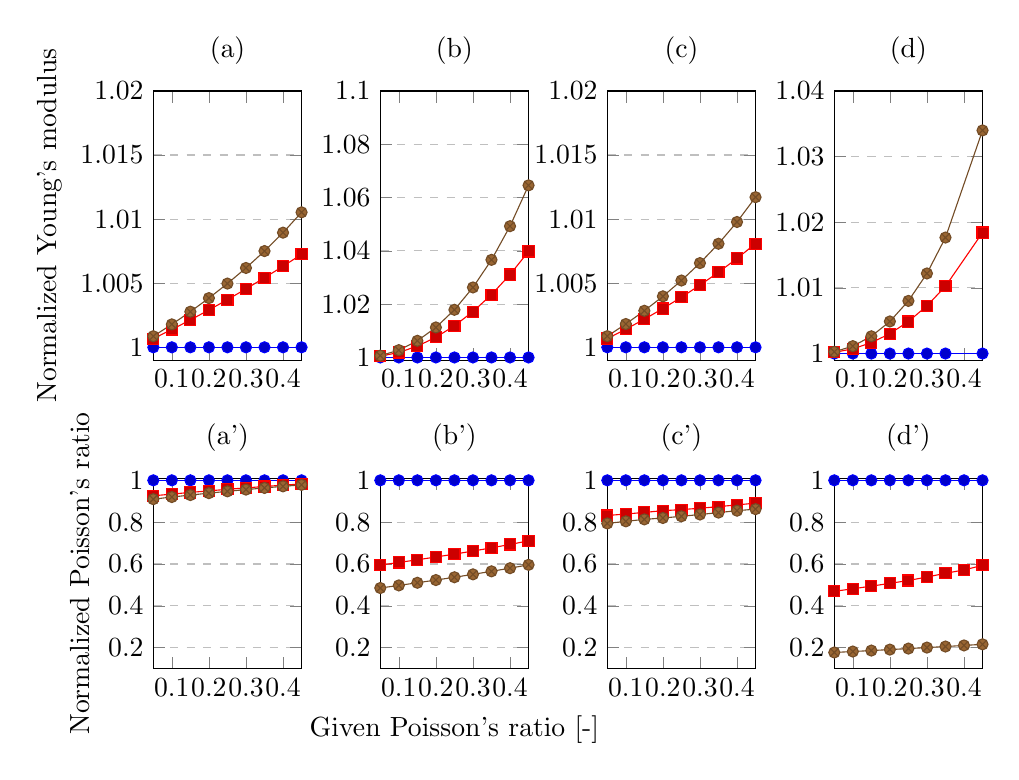
\begin{tikzpicture}[scale=1]

\pgfplotstableread{
nuxy	tr0	tr0.1	trINF
0.05	1	1.000678	1.000864
0.1	1	1.00139	1.00179
0.15	1	1.002135	1.002779
0.2	1	1.002912	1.003838
0.25	1	1.003719	1.004972
0.3	1	1.004556	1.00619
0.35	1	1.005424	1.007508
0.4	1	1.006323	1.008945
0.45	1	1.007256	1.010531

}\totarea

\pgfplotstableread{
nuxy	tr0	tr0.1	trINF	
0.05	1	1.00047	1.00068
0.1	1	1.00188	1.00275
0.15	1	1.00424	1.00625
0.2	1	1.00757	1.01126
0.25	1	1.01188	1.01788
0.3	1	1.01721	1.02627
0.35	1	1.02359	1.03663
0.4	1	1.0311	1.04926
0.45	1	1.03978	1.06458

}\chosenarea

\pgfplotstableread{
nuxy	tr0	tr0.1	trINF	
0.05	1	1.000683	1.000869
0.1	1	1.001413	1.001817
0.15	1	1.002193	1.00285
0.2	1	1.003024	1.003977
0.25	1	1.003908	1.005211
0.3	1	1.00485	1.006571
0.35	1	1.005855	1.00808
0.4	1	1.006931	1.009777
0.45	1	1.008091	1.011712



}\experiment


\pgfplotstableread{
nuxy	tr0	tr0.1	trINF	
0.05	1	1.00018	1.00027
0.1	1	1.00072	1.00113
0.15	1	1.00166	1.00263
0.2	1	1.00303	1.00489
0.25	1	1.00488	1.00802
0.3	1	1.00727	1.0122
0.35	1	1.01025	1.01767
0.45	1	1.01843	1.03399




}\experimentBasic

\pgfplotstableread{
nuxy	tr0	tr0.1	trINF	i0	i0.1	iINF
0.05	1	0.59508	0.48536	1	0.9382	0.8238
0.1	1	0.60748	0.49784	1	0.942	0.8349
0.15	1	0.62028	0.51052	1	0.946266667	0.846
0.2	1	0.63358	0.52349	1	0.951	0.8571
0.25	1	0.64744	0.53684	1	0.95616	0.86792
0.3	1	0.66198	0.55067	1	0.961866667	0.878266667
0.35	1	0.67731	0.56509	1	0.968228571	0.887942857
0.4	1	0.69357	0.58022	1	0.975575	0.89565
0.45	1	0.7109	0.5962	1	0.984644444	0.8698


}\nutotarea

\pgfplotstableread{
nuxy	tr0	tr0.1	trINF	i0	i0.1	iINF
0.05	1	0.926	0.91	1	0.9812	0.9456
0.1	1	0.9342	0.9201	1	0.9847	0.9552
0.15	1	0.9422	0.9296	1	0.988066667	0.964666667
0.2	1	0.94975	0.9387	1	0.99145	0.97405
0.25	1	0.95704	0.9474	1	0.99464	0.98336
0.3	1	0.963933333	0.9557	1	0.997766667	0.992733333
0.35	1	0.970542857	0.963628571	1	1.000742857	1.002171429
0.4	1	0.9768	0.971175	1	1.00355	1.011925
0.45	1	0.982755556	0.978377778	1	1.006288889	1.022933333

}\nuchosenarea

\pgfplotstableread{
nuxy	tr0	tr0.1	trINF	i0	i0.1	iINF
0.05	1	0.832	0.794	1	0.938	0.818
0.1	1	0.839	0.804	1	0.941	0.825
0.15	1	0.846666667	0.813333333	1	0.946666667	0.833333333
0.2	1	0.855	0.82	1	0.95	0.84
0.25	1	0.86	0.828	1	0.956	0.852
0.3	1	0.866666667	0.836666667	1	0.96	0.866666667
0.35	1	0.874285714	0.845714286	1	0.968571429	0.882857143
0.4	1	0.8825	0.855	1	0.975	0.905
0.45	1	0.891111111	0.862222222	1	0.984444444	0.931111111

}\nuexperiment


\pgfplotstableread{
nuxy	tr0	tr0.1	trINF	
0.05	1	0.469722892	0.177420121
0.1	1	0.481606855	0.181931174
0.15	1	0.494385965	0.186522064
0.2	1	0.507614213	0.191215676
0.25	1	0.521384929	0.196042474
0.3	1	0.537963909	0.200827288
0.35	1	0.555636789	0.205808631
0.4	1	0.571794872	0.211041361
0.45	1	0.593810666	0.216371772


}\nuexperimentBasic

%plot transv iso total area DSP

\begin{axis}[
name=b1,height=5cm,width=\textwidth/3.5,
    title={(a)},
%    xlabel={Temperature [\textcelsius]},
    ylabel={Normalized Young's modulus},
    xmin=0.05, xmax=0.45,
    ymin=0.999, ymax=1.02,
        yticklabel style={/pgf/number format/fixed,
                  /pgf/number format/precision=3},
%     xtick={1,...,9},
%    ytick={0,20,40,60,80},
%     xticklabels={$K=0$,$K=0.001$,$K=0.01$,$K=0.1$,$K=1$, $K=10$, $K=100$,
%     $K=1000$, $K=\infty$}, 
%     x tick label style={
%     rotate=60,anchor=east},
    ymajorgrids=true,
    grid style=dashed,
]
% \end{axis}    
% \begin{axis}[legend pos=outer north east]
 
 
    \addplot table[x=nuxy,y=tr0	] {\totarea}; \label{k1}
%     \addlegendentry{$\nu$=0.05}
    \addplot table[x=nuxy,y=tr0.1 ] {\totarea}; \label{k2}
%     \addlegendentry{$\nu$=0.1}
    \addplot table[x=nuxy,y=trINF ] {\totarea}; \label{k3}
%     \addlegendentry{$\nu$=0.15}

\end{axis}


%plot transviso chosen area  DSP

\begin{axis}[legend pos=outer north east,
	name=b2,at={($(b1.east)+(1cm,0)$)},anchor=west, height=5cm,
	width=\textwidth/3.5, title={(b)},
% xlabel={Poisson's ratio [-]},
%    ylabel={Measured stiffness [Pa]},
    xmin=0.05, xmax=0.45,
    ymin=0.999, ymax=1.1,
    yticklabel style={/pgf/number format/fixed,
                  /pgf/number format/precision=4},
%     xtick={1,...,9},
%    ytick={0,20,40,60,80},
%     xticklabels={$K=0$,$K=0.001$,$K=0.01$,$K=0.1$,$K=1$, $K=10$, $K=100$,
%     $K=1000$, $K=\infty$},
%     x tick label style={
%         rotate=60,anchor=east},
    ymajorgrids=true,
    grid style=dashed,
%     scaled y ticks=base 10:3,
    bar shift=0pt
]

    \addplot table[x=nuxy,y=tr0	] {\chosenarea}; \label{k1}
%     \addlegendentry{$\nu$=0.05}
    \addplot table[x=nuxy,y=tr0.1 ] {\chosenarea}; \label{k2}
%     \addlegendentry{$\nu$=0.1}
    \addplot table[x=nuxy,y=trINF ] {\chosenarea}; \label{k3}
%     \addlegendentry{$\nu$=0.15}

%Experimental approach

\end{axis}


\begin{axis}[legend pos=outer north east,
	name=b3,at={($(b2.east)+(1cm,0)$)},anchor=west,
	height=5cm,width=\textwidth/3.5, title={(c)},
%    xlabel={Temperature [\textcelsius]},
%    ylabel={Measured stiffness [Pa]},
    xmin=0.05, xmax=0.45,
    ymin=0.999, ymax=1.02,
    yticklabel style={/pgf/number format/fixed,
                  /pgf/number format/precision=3},
%     xtick={1,...,9},
%    ytick={0,20,40,60,80},
%     xticklabels={$K=0$,$K=0.001$,$K=0.01$,$K=0.1$,$K=1$, $K=10$, $K=100$,
%     $K=1000$, $K=\infty$},
%     x tick label style={
%         rotate=60,anchor=east},
    ymajorgrids=true,
    grid style=dashed,
    bar shift=0pt
]

    \addplot table[x=nuxy,y=tr0	] {\experiment}; \label{k1}
%     \addlegendentry{$\nu$=0.05}
    \addplot table[x=nuxy,y=tr0.1 ] {\experiment}; \label{k2}
%     \addlegendentry{$\nu$=0.1}
    \addplot table[x=nuxy,y=trINF ] {\experiment}; \label{k3}
%     \addlegendentry{$\nu$=0.15}




\end{axis}


\begin{axis}[legend pos=outer north east,
	name=b3a,at={($(b3.east)+(1cm,0)$)},anchor=west,
	height=5cm,width=\textwidth/3.5, title={(d)},
%    xlabel={Temperature [\textcelsius]},
%    ylabel={Measured stiffness [Pa]},
    xmin=0.05, xmax=0.45,
    ymin=0.999, ymax=1.04,
    yticklabel style={/pgf/number format/fixed,
                  /pgf/number format/precision=3},
%     xtick={1,...,9},
%    ytick={0,20,40,60,80},
%     xticklabels={$K=0$,$K=0.001$,$K=0.01$,$K=0.1$,$K=1$, $K=10$, $K=100$,
%     $K=1000$, $K=\infty$},
%     x tick label style={
%         rotate=60,anchor=east},
    ymajorgrids=true,
    grid style=dashed,
    bar shift=0pt
]

    \addplot table[x=nuxy,y=tr0	] {\experimentBasic}; \label{k1}
%     \addlegendentry{$\nu$=0.05}
    \addplot table[x=nuxy,y=tr0.1 ] {\experimentBasic}; \label{k2}
%     \addlegendentry{$\nu$=0.1}
    \addplot table[x=nuxy,y=trINF ] {\experimentBasic}; \label{k3}
%     \addlegendentry{$\nu$=0.15}




\end{axis}

\begin{axis}
[name=b4,at={($(b2.south)-(0,1.5cm)$)},anchor=north,
height=4cm,width=\textwidth/3.5, title={(b')},
    xlabel={Given Poisson's ratio [-]},
%     ylabel={Error Poisson's ratio},
    xmin=0.05, xmax=0.45,
    ymin=0.1, ymax=1.01,
        yticklabel style={/pgf/number format/fixed,
                  /pgf/number format/precision=3},
%     xtick={1,...,9},
%    ytick={0,20,40,60,80},
%     xticklabels={$K=0$,$K=0.001$,$K=0.01$,$K=0.1$,$K=1$, $K=10$, $K=100$,
%     $K=1000$, $K=\infty$}, 
%     x tick label style={
%     rotate=60,anchor=east},
    ymajorgrids=true,
    grid style=dashed,
]
% \end{axis}    
% \begin{axis}[legend pos=outer north east]
 
 
    \addplot table[x=nuxy,y=tr0	] {\nutotarea}; \label{nuk1}
%     \addlegendentry{$\nu$=0.05}
    \addplot table[x=nuxy,y=tr0.1 ] {\nutotarea}; \label{nuk2}
%     \addlegendentry{$\nu$=0.1}
    \addplot table[x=nuxy,y=trINF ] {\nutotarea}; \label{nuk3}
%     \addlegendentry{$\nu$=0.15}

\end{axis}


% plot transviso chosen area  DSP

\begin{axis}[
	name=b5,at={($(b1.south)-(0,1.5cm)$)},anchor=north, height=4cm,
	width=\textwidth/3.5, title={(a')},
%     xlabel={Given Poisson's ratio [-]},
   ylabel={Normalized Poisson's ratio},
    xmin=0.05, xmax=0.45,
    ymin=0.1, ymax=1.01,
%     yticklabel style={/pgf/number format/fixed,
%                   /pgf/number format/precision=3},
%     xtick={1,...,9},
%    ytick={0,20,40,60,80},
%     xticklabels={$0.05$,$0.3$,,,$0.45$},
%     x tick label style={
%         rotate=60,anchor=east},
    ymajorgrids=true,
    grid style=dashed,
    bar shift=0pt
]

    \addplot table[x=nuxy,y=tr0	] {\nuchosenarea}; \label{nuk1}
%     \addlegendentry{$\nu$=0.05}
    \addplot table[x=nuxy,y=tr0.1 ] {\nuchosenarea}; \label{nuk2}
%     \addlegendentry{$\nu$=0.1}
    \addplot table[x=nuxy,y=trINF ] {\nuchosenarea}; \label{nuk3}
%     \addlegendentry{$\nu$=0.15}

%Experimental approach

\end{axis}


\begin{axis}[name=b6,at={($(b3.south)-(0,1.5cm)$)},anchor=north,
height=4cm,width=\textwidth/3.5, title={(c')},
%    xlabel={Temperature [\textcelsius]},
%    ylabel={Measured stiffness [Pa]},
    xmin=0.05, xmax=0.45,
    ymin=0.1, ymax=1.01,
%     yticklabel style={/pgf/number format/fixed,
%                   /pgf/number format/precision=3},
%     xtick={1,...,9},
%    ytick={0,20,40,60,80},
%     xticklabels={$K=0$,$K=0.001$,$K=0.01$,$K=0.1$,$K=1$, $K=10$, $K=100$,
%     $K=1000$, $K=\infty$},
%     x tick label style={
%         rotate=60,anchor=east},
    ymajorgrids=true,
    grid style=dashed,
    bar shift=0pt
]

    \addplot table[x=nuxy,y=tr0	] {\nuexperiment}; \label{nuk1}
%     \addlegendentry{$\nu$=0.05}
    \addplot table[x=nuxy,y=tr0.1 ] {\nuexperiment}; \label{nuk2}
%     \addlegendentry{$\nu$=0.1}
    \addplot table[x=nuxy,y=trINF ] {\nuexperiment}; \label{nuk3}
%     \addlegendentry{$\nu$=0.15}




\end{axis}

\begin{axis}
[name=b6a,at={($(b3a.south)-(0,1.5cm)$)},anchor=north,
height=4cm,width=\textwidth/3.5, title={(d')},
%    xlabel={Temperature [\textcelsius]},
%    ylabel={Measured stiffness [Pa]},
    xmin=0.05, xmax=0.45,
    ymin=0.1, ymax=1.01,
%     yticklabel style={/pgf/number format/fixed,
%                   /pgf/number format/precision=3},
%     xtick={1,...,9},
%    ytick={0,20,40,60,80},
%     xticklabels={$K=0$,$K=0.001$,$K=0.01$,$K=0.1$,$K=1$, $K=10$, $K=100$,
%     $K=1000$, $K=\infty$},
%     x tick label style={
%         rotate=60,anchor=east},
    ymajorgrids=true,
    grid style=dashed,
    bar shift=0pt
]

    \addplot table[x=nuxy,y=tr0	] {\nuexperimentBasic}; \label{nuk1}
%     \addlegendentry{$\nu$=0.05}
    \addplot table[x=nuxy,y=tr0.1 ] {\nuexperimentBasic}; \label{nuk2}
%     \addlegendentry{$\nu$=0.1}
    \addplot table[x=nuxy,y=trINF ] {\nuexperimentBasic}; \label{nuk3}
%     \addlegendentry{$\nu$=0.15}




\end{axis}


\end{tikzpicture}

\captionsetup{justification=centering}
\caption{Normalizad Young's moduli of transversely isotropic
material for spring constant $K=0$ (\ref{k1}) gliding, $K=0.1$ (\ref{k2})
intermediate and $K=\infty$ (\ref{k3}) no slipping vs.
different given Poisson's ratio ($\nu$) values for a) chosen area of
interest, b) total area of interest and c) experimental methodology.
d) Basic methodology from strain obtaint from the testing mashine plates
displacement a') Normalized Poisson's ratio values of material with different
given Poisson's ratio ($\nu$) values for chosen area of
interest, b') total area of interest c') experimental methodology d) Basic methodology from strain obtaint from the testing mashine plates
displacement with the manual transverse displacement measurement.}
\label{fig:strainmethods}


\end{figure}
\end{center}



In the second approach only the middle 50\% of the area part was
taken for determination of strain. The plot in Figure \ref{fig:strainmethods}$a$
shows that with this method the Young's moduli is less overestimated.\par
  In the last approach where ASTM-D143-94 standard
with strain gauge technique was used, the error is very close to the one in
second approach. The plot in Figure \ref{fig:strainmethods}$c$ depicts that.
This is due to the strain is measured between two points in the center of 
the sample where the constraining effect is less severe. 

\begin{figure}[h]
\centering
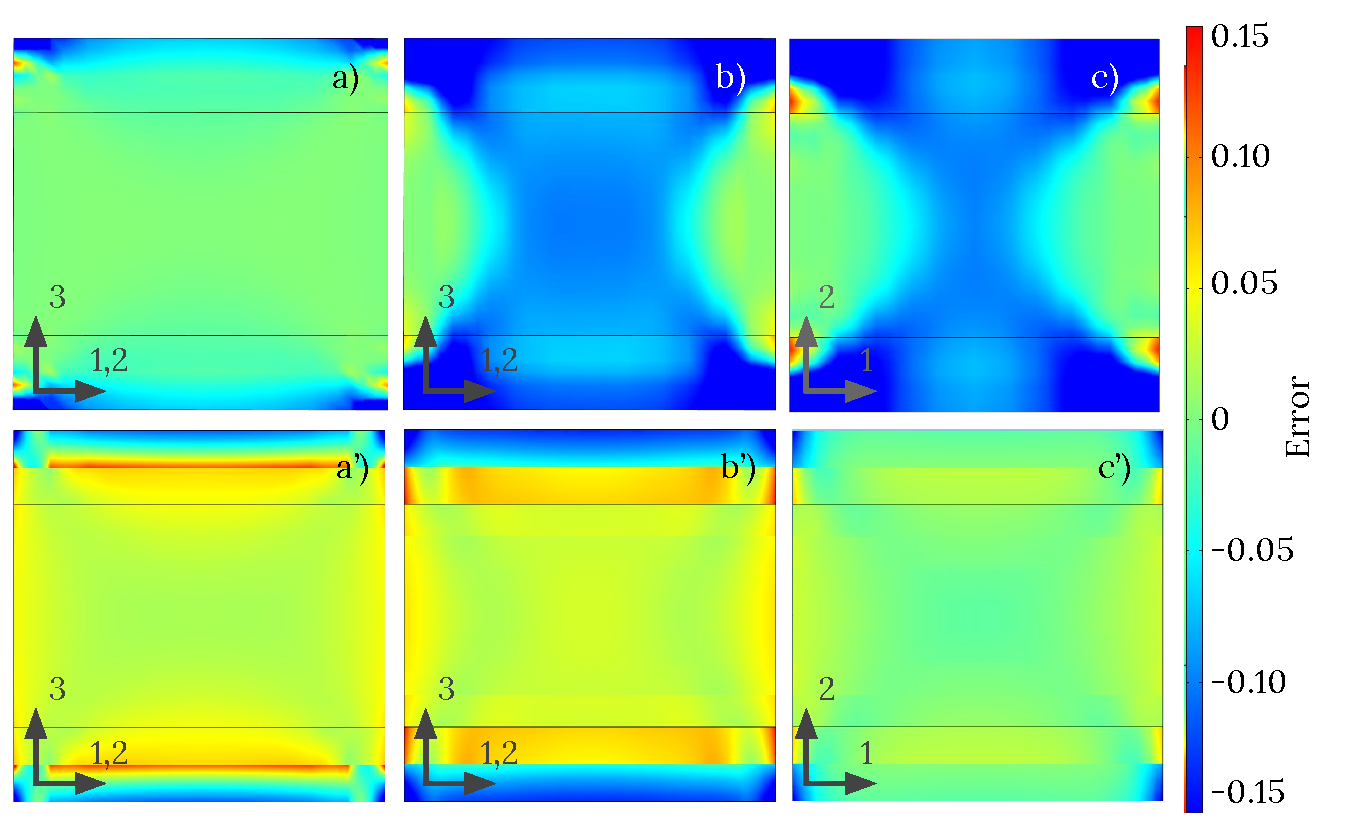
\includegraphics[width=\textwidth]{BarellingError.pdf}
\label{fig:Error}
\caption{\label{fig:Error} a) Simulated results of error for measured Young's
moduli ($E$) of Isotropic, b) transversely Isotropic material ($E_L$) and for
transversely Isotropic material ($E_T$) in c). 
a') Simulated results of error for measured
Poisson's ratio ($\nu$) of Isotropic, b')
transversely isotropic material ($\nu_{LT}$) and c') transversely isotropic
material plane ($\nu_{TT}$).($K=0.1;\nu=0.3$)}

\end{figure}

Large error values for the Young's
modulus close to the horizontal edges of isotropic model are clearly visible in
Figure \ref{fig:Error}$a$. The opposite is true for the transversely isotropic
sample in (Figure \ref{fig:Error}$b,c$), for $LT$ plane 
the Young's moduli in the central area is overestimated whereas for $TT$ plane
the strain field looks similar to the isotropic material.\par
These simulations are supporting the experimental results in Figure
\ref{fig:explot}. Where the average strain diagram for the total area is showing larger Young's moduli than
the one for the chosen area.
Additional outcomes are deduced  while observing the error fields in Figure
\ref{fig:Error}$a'-c'$. The ASTM-D143-94 standard \cite{american2009standard} requires
installation of strain gauges in the center of the sample. This approach will
lead to underestimation of Poisson's ratio in transversely isotropic cubic
sample due to the barrelling formation. On the other hand accurate values will
be obtained for the isotropic material, where the constraining effect influence
the horizontal edges of the sample. The chosen central area of the isotropic
sample is most favourable for accurate measurements.


\begin{description}
\item{\textit{Barrelling in orthotropic material}}
\end{description}
As it was mentioned, the barreling is more severe in the isotropic material and
less in transverse isotropic. To check whether this stands for the orthotropic
materials, a true orthotropic model was simulated, based on wood material properties
that were experimentally determined \cite{vorobyevcharacterisation}. \par

\begin{center}% note that \centering uses less vspace...
\begin{figure}[h]
\pgfplotsset{every axis legend/.append style={
		at={(0.5,1.03)},
		anchor=north}}

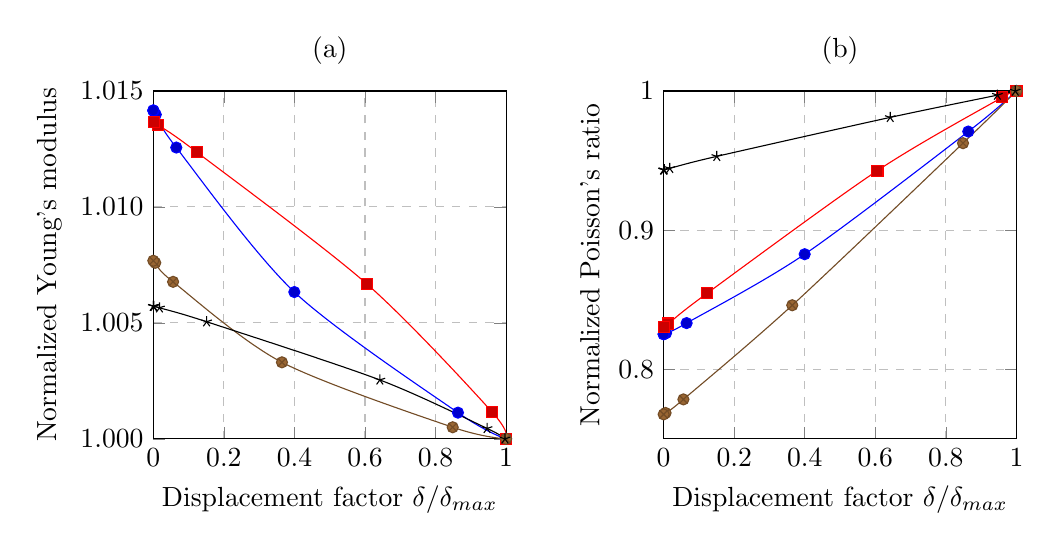
\begin{tikzpicture}[scale=1]

	\pgfplotstableread{
K	ZY	dZY	ZX	dZX	XZ	dXZ	XY	dXY
0	1	0.99931	1	1	1	1	1	0.99666
0.001	1.00113	0.86336	1.00116	0.95989	1.0005	0.84846	1.00045	0.94592
0.01	1.00633	0.39972	1.00667	0.60587	1.0033	0.36457	1.00254	6.42E-01
0.1	1.01256	0.06514	1.01236	0.12346	1.00677	0.05606	1.00505	1.51E-01
1	1.01398	0.00698	1.01353	0.01348	1.00759	0.0055	1.00565	1.74E-02
10	1.01414	0.000703066	1.01365	0.00103	1.00768	0.000058874	1.00571	0.00177
100	1.01416	7.03579E-05	1.01367	-0.000226463	1.00769	-0.000489077	1.00572	0.000176984
1000	1.01416	7.0363E-06	1.01367	-0.000352727	1.00769	-0.000543916	1.00572	1.77012E-05


}\datatable

\pgfplotstableread{
K	ZY	dZY	ZX	dZX	XZ	dXZ	XY	dXY
0	1	1	0.99999	1	0.99996	1	0.99996	0.99666
0.001	0.97083	0.86336	0.99543	0.95989	0.96247	0.84846	9.97E-01	0.94592
0.01	0.88268	0.39972	0.94277	0.60587	0.84601	0.36457	9.81E-01	0.64214
0.1	0.83318	0.06514	0.85465	0.12346	0.77836	0.05606	9.53E-01	0.15068
1	0.82602	0.00698	0.83283	0.01348	0.7686	0.0055	0.9444	0.0174
10	0.82528	0.000703066	0.8303	0.00103	0.76759	0.000058874	0.94339	0.00177
100	0.8252	7.03579E-05	0.83005	-0.000226463	0.76749	-0.000489077	0.94328	0.000176984
1000	0.82519	7.0363E-06	0.83002	-0.000352727	0.76748	-0.000543916	0.94327	1.77012E-05



}\datatableA




\begin{axis}[
name=plot0,height=6cm,width=\textwidth/2,
    title={(a)},
	xlabel={Displacement factor $\delta/\delta_{max}$},
    ylabel={Normalized Young's modulus},
    xmin=0, xmax=1,
    ymin=1, ymax=1.015,
%     xtick={1,...,9},
%     xticklabels={$0$,$0.001$,$0.01$,$0.1$,$1$, $10$, $100$,
%     $1000$, $\infty$}, 
%         x tick label style={yshift=-1ex,
%         rotate=45,anchor=east		},
    y tick label style={
        /pgf/number format/.cd,
            fixed,
            fixed zerofill,
            precision=3,
        /tikz/.cd},
%     ytick={0,1.01,1.015,1.02,1.025},
    ymajorgrids=true,
    xmajorgrids=true,
    grid style=dashed,
]
% \end{axis}    
% \begin{axis}[legend pos=outer north east]
 
 
    \addplot+[smooth] table[x=dZY,y=ZY] {\datatable};
%     \addlegendentry{$\nu$=0.05}
    \addplot+[smooth] table[x=dZX,y=ZX] {\datatable};
%     \addlegendentry{$\nu$=0.1}
    \addplot+[smooth] table[x=dXZ,y=XZ] {\datatable};
%     \addlegendentry{$\nu$=0.15}
    \addplot+[smooth] table[x=dXY,y=XY] {\datatable};

\end{axis}

\begin{axis}[
name=plot1,at={($(plot0.east)+(2cm,0)$)},anchor=west,
height=6cm,width=\textwidth/2, title={(b)},
	xlabel={Displacement factor $\delta/\delta_{max}$},
    ylabel={Normalized Poisson's ratio},
    xmin=0, xmax=1,
    ymin=0.75, ymax=1,
    yticklabel style={/pgf/number format/fixed,
                  /pgf/number format/precision=3},
%     xtick={1,...,9},
%    ytick={0,20,40,60,80},
%     xticklabels={$0$,$0.001$,$0.01$,$0.1$,$1$, $10$, $100$,
%     $1000$, $\infty$},
%             x tick label style={yshift=-1ex,
%         rotate=45,anchor=east		}, 
    ymajorgrids=true,
    xmajorgrids=true,
    grid style=dashed,
    bar shift=0pt
]

    \addplot+[smooth] table[x=dZY,y=ZY] {\datatableA}; \label{VasaZY}
%     \addlegendentry{$\nu$=0.05}
    \addplot+[smooth] table[x=dZX,y=ZX] {\datatableA}; \label{VasaZX}
%     \addlegendentry{$\nu$=0.1}
    \addplot+[smooth] table[x=dXZ,y=XZ] {\datatableA}; \label{VasaXZ}
%     \addlegendentry{$\nu$=0.15}
    \addplot+[smooth] table[x=dXY,y=XY] {\datatableA}; \label{VasaXY}



\end{axis}


\end{tikzpicture}


\captionsetup{justification=centering}
\caption{Simulated and normalized results based on experiment of
orthotropic material. a) Young's moduli and b) Poisson's ratio while measuring
chosen strain field from directions $LT$(\ref{VasaZY}),
$LR$(\ref{VasaZX}), 
$TL$(\ref{VasaXZ}), 
$TR$(\ref{VasaXY}).}


\label{fig:ortho}
\end{figure}

\end{center}

The results is for normalised Young's moduli in all wood orthotropic directions and Poisson's ratio versus the displacement factor are plotted in Figure \ref{fig:ortho}. The notation for the wood planes in Figure is corresponding to the wood principal orthotropic directions, where Longitudinal $(L)$, Radial $R$, Tangential $T$. \par It shows that the magnitude of error is less than those for the transversely isotropic material. 
In case of identifying the Young's moduli $E_L$, plane  $LT$ might be
beneficial. This is due to the less slope of $LT$ curve in comparison to $LR$ in
Figure \ref{fig:ortho}a. \par
As for transversely isotropic material the Poisson's ratio is underestimated
with the increasing constraining effect the same is observed for the orthotropic
material simulation. The magnitude of error is spread, however the $\nu_{LT}$,
$\nu_{LR}$, $\nu_{TR}$ are less influenced by the barrelling. Contrary
$\nu_{TL}$ is more underestimated than the others, presented in Figure
\ref{fig:ortho}b. When $L$
direction is in transverse plane, the geometrical response is less significant
because of its stiffness. Therefore the magnitude of possible error depending on
barrelling is larger. However having the $\nu_{LT}$,
$\nu_{LR}$, $\nu_{TR}$ ratios the symmetry principle can
be used to determine the rest.







%poisson's vs poisson's dependency
% \color{black}
% 
% \begin{center}
% \begin{figure}[!ht]
% \pgfplotsset{every axis legend/.append style={
% 		at={(0.5,1.03)},
% 		anchor=north}}
% 
% \begin{tikzpicture}[scale=1]
% 
% \pgfplotstableread{
% nuxy	tr0	tr0.1	trINF	i0	i0.1	iINF
% 0.05	0.05	0.04161	0.03981	0.05	0.04691	0.04119
% 0.1	0.1	0.08404	0.08063	0.1	0.0942	0.08349
% 0.15	0.15	0.12728	0.1224	0.15	0.14194	0.1269
% 0.2	0.2	0.1713	0.16507	0.2	0.1902	0.17142
% 0.25	0.25	0.21607	0.2086	0.25	0.23904	0.21698
% 0.3	0.3	0.26158	0.25295	0.3	0.28856	0.26348
% 0.35	0.35	0.30782	0.29808	0.35	0.33888	0.31078
% 0.4	0.4	0.35479	0.34396	0.4	0.39023	0.35826
% 0.45	0.45	0.40251	0.39058	0.45	0.44309	0.39141
% 
% }\nutotarea
% 
% \pgfplotstableread{
% nuxy	tr0	tr0.1	trINF	i0	i0.1	iINF
% 0.05	0.05	0.0463	0.0455	0.05	0.04906	0.04728
% 0.1	0.1	0.09342	0.09201	0.1	0.09847	0.09552
% 0.15	0.15	0.14133	0.13944	0.15	0.14821	0.1447
% 0.2	0.2	0.18995	0.18774	0.2	0.19829	0.19481
% 0.25	0.25	0.23926	0.23685	0.25	0.24866	0.24584
% 0.3	0.3	0.28918	0.28671	0.3	0.29933	0.29782
% 0.35	0.35	0.33969	0.33727	0.35	0.35026	0.35076
% 0.4	0.4	0.39072	0.38847	0.4	0.40142	0.40477
% 0.45	0.45	0.44224	0.44027	0.45	0.45283	0.46032
% }\nuchosenarea
% 
% \pgfplotstableread{
% nuxy	tr0	tr0.1	trINF	i0	i0.1	iINF
% 0.05	0.05	0.0416	0.03970	0.05	0.04690	0.04090
% 0.1	0.1	0.0839	0.08040	0.1	0.09410	0.08250
% 0.15	0.15	0.127	0.12200	0.15	0.14200	0.12500
% 0.2	0.2	0.171	0.16400	0.2	0.19000	0.16800
% 0.25	0.25	0.215	0.20700	0.25	0.23900	0.21300
% 0.3	0.3	0.26	0.25100	0.3	0.28800	0.26000
% 0.35	0.35	0.306	0.29600	0.35	0.33900	0.30900
% 0.4	0.4	0.353	0.34200	0.4	0.39000	0.36200
% 0.45	0.45	0.401	0.38800	0.45	0.44300	0.41900
% 
% }\nuexperiment
% 
% 
% 
% 
% \begin{axis}[
% name=c1,height=4cm,width=4cm,
%     title={a)},
% %    xlabel={Temperature [\textcelsius]},
%     ylabel={Measured Poisson's ratio [-]},
%     xmin=0.05, xmax=0.45,
%     ymin=0.05, ymax=0.45,
%         yticklabel style={/pgf/number format/fixed,
%                   /pgf/number format/precision=3},
% %     xtick={1,...,9},
% %    ytick={0,20,40,60,80},
% %     xticklabels={$K=0$,$K=0.001$,$K=0.01$,$K=0.1$,$K=1$, $K=10$, $K=100$,
% %     $K=1000$, $K=\infty$}, 
% %     x tick label style={
% %     rotate=60,anchor=east},
%     ymajorgrids=true,
%     grid style=dashed,
% ]
% % \end{axis}    
% % \begin{axis}[legend pos=outer north east]
%  
%  
%     \addplot table[x=nuxy,y=tr0	] {\nutotarea}; \label{nuk1}
% %     \addlegendentry{$\nu$=0.05}
%     \addplot table[x=nuxy,y=tr0.1 ] {\nutotarea}; \label{nuk2}
% %     \addlegendentry{$\nu$=0.1}
%     \addplot table[x=nuxy,y=trINF ] {\nutotarea}; \label{nuk3}
% %     \addlegendentry{$\nu$=0.15}
% 
% \end{axis}
% 
% 
% % plot transviso chosen area  DSP
% 
% \begin{axis}[legend pos=outer north east,
% 	name=c2,at={($(c1.east)+(1cm,0)$)},anchor=west, height=4cm, width=4cm,
%     title={b)},
%     xlabel={Given Poisson's ratio [-]},
% %    ylabel={Measured stiffness [Pa]},
%     xmin=0.05, xmax=0.45,
%     ymin=0.05, ymax=0.45,
% %     yticklabel style={/pgf/number format/fixed,
% %                   /pgf/number format/precision=3},
% %     xtick={1,...,9},
% %    ytick={0,20,40,60,80},
% %     xticklabels={$K=0$,$K=0.001$,$K=0.01$,$K=0.1$,$K=1$, $K=10$, $K=100$,
% %     $K=1000$, $K=\infty$},
% %     x tick label style={
% %         rotate=60,anchor=east},
%     ymajorgrids=true,
%     grid style=dashed,
%     bar shift=0pt
% ]
% 
%     \addplot table[x=nuxy,y=tr0	] {\nuchosenarea}; \label{nuk1}
% %     \addlegendentry{$\nu$=0.05}
%     \addplot table[x=nuxy,y=tr0.1 ] {\nuchosenarea}; \label{nuk2}
% %     \addlegendentry{$\nu$=0.1}
%     \addplot table[x=nuxy,y=trINF ] {\nuchosenarea}; \label{nuk3}
% %     \addlegendentry{$\nu$=0.15}
% 
% %Experimental approach
% 
% \end{axis}
% 
% 
% \begin{axis}[legend pos=outer north east,
% 	name=c3,at={($(c2.east)+(1cm,0)$)},anchor=west, height=4cm,width=4cm,
%     title={c)},
% %    xlabel={Temperature [\textcelsius]},
% %    ylabel={Measured stiffness [Pa]},
%     xmin=0.05, xmax=0.45,
%     ymin=0.05, ymax=0.45,
% %     yticklabel style={/pgf/number format/fixed,
% %                   /pgf/number format/precision=3},
% %     xtick={1,...,9},
% %    ytick={0,20,40,60,80},
% %     xticklabels={$K=0$,$K=0.001$,$K=0.01$,$K=0.1$,$K=1$, $K=10$, $K=100$,
% %     $K=1000$, $K=\infty$},
% %     x tick label style={
% %         rotate=60,anchor=east},
%     ymajorgrids=true,
%     grid style=dashed,
%     bar shift=0pt
% ]
% 
%     \addplot table[x=nuxy,y=tr0	] {\nuexperiment}; \label{nuk1}
% %     \addlegendentry{$\nu$=0.05}
%     \addplot table[x=nuxy,y=tr0.1 ] {\nuexperiment}; \label{nuk2}
% %     \addlegendentry{$\nu$=0.1}
%     \addplot table[x=nuxy,y=trINF ] {\nuexperiment}; \label{nuk3}
% %     \addlegendentry{$\nu$=0.15}
% 
% 
% 
% 
% \end{axis}
% 
% 
% \end{tikzpicture}
% \captionsetup{justification=centering}
% \caption{Measured vs. given Poisson's ratio
% ($\nu_{31}$, $\nu_{32}$) in transverse-isotropic material for spring
% coefficients $K=0$ (\ref{k1}), $K=0.1$ (\ref{k2}) and $K=\infty$ (\ref{k3});\\
% \color{red}{a) total area of interest, b) chosen area of interest c)
% experiment.}}
% 
% 
% \end{figure}
% \end{center}






% \begin{figure}[!ht]
% \centering
% \pgfplotsset{every axis legend/.append style={
% 		at={(0.5,1.03)},
% 		anchor=north}}
% 
% \begin{tikzpicture}
%  [spy using outlines={circle,black,magnification=3,size=1cm,
%  connect spies}]
% % Data for the plot showing the stability and independency of Emod
% 
% \pgfplotstableread{
% Emodgiven	nul	tr0.1	iso0.1	trinf	isoinf
% 1	1	1.00638	1.02469	1.00797	0.89131
% 2	2	2.01276	2.04938	2.01595	1.78262
% 3	3	3.01914	3.07408	3.02392	2.67393
% 4	4	4.02551	4.09877	4.0319	3.56524
% 5	5	5.03189	5.12346	5.03987	4.45655
% }\emodgivread
% 
% 
% 
% \begin{axis}[
% name=c1,height=5cm,width=5cm,
%     title={a)},
%     xlabel={Given Young's modulus [Pa]},
%     ylabel={Measured Young's modulus [Pa]},
%     xmin=1, xmax=5.2,
%     ymin=1, ymax=5.2,
%         yticklabel style={/pgf/number format/fixed,
%                   /pgf/number format/precision=3},
% %     xtick={1,...,9},
% %    ytick={0,20,40,60,80},
% %     xticklabels={$K=0$,$K=0.001$,$K=0.01$,$K=0.1$,$K=1$, $K=10$, $K=100$,
% %     $K=1000$, $K=\infty$}, 
% %     x tick label style={
% %     rotate=60,anchor=east},
%     ymajorgrids=true,
%     grid style=dashed,
% ]
% 
%     \addplot[mark=otimes, green, solid] table[x=Emodgiven,y=nul	]
%     {\emodgivread};
%     \label{e1}
% %     \addlegendentry{$\nu$=0.05}
%     \addplot [mark=x, darkgray,    ] table[x=Emodgiven,y=tr0.1 ]
%     {\emodgivread}; \label{e2}
% %     \addlegendentry{$\nu$=0.1}
%     \addplot [mark=x, gray,  ] table[x=Emodgiven,y=trinf ]
%     {\emodgivread};
%     \label{e3}
% %     \addlegendentry{$\nu$=0.15}
%     \addplot [mark=o, red  ] table[x=Emodgiven,y=iso0.1 ]
%     {\emodgivread};
%     \label{e4}
% %     \addlegendentry{$\nu$=0.1}
%     \addplot [mark=o, red    ] table[x=Emodgiven,y=isoinf ]
%     {\emodgivread};
%     \label{e5}
% %     \addlegendentry{$\nu$=0.15}
% 
% \coordinate (spypoint) at (axis cs:4,4);
% \coordinate (magnifyglass) at (axis cs:2.2,3.8);
% 
% \end{axis}
% 
% % \spy on (2.5,2.5) in node [left] at (1.25,1.75);
% \spy [gray, size=1.5cm] on (spypoint)
%    in node[fill=white] at (magnifyglass);
% 
% \end{tikzpicture}
% \captionsetup{justification=centering}
% \caption{Measured vs. given stiffness
% ($E_{1}$) in transverse-isotropic(\ref{e2}) and isotropic(\ref{e4}) material for
% spring coefficients $K=0$ (\ref{e1}), $K=0.1$ (\ref{e2}, \ref{e4}) and
% $K=\infty$ (\ref{e3}, \ref{e5});\\
% \color{red}{a) total area of interest, b) chosen area of interest c)
% experiment.}}
% 
% 
% \end{figure}







\section{Conclusions}

The barrelling formation in cubic samples is an artifact that can influence the
estimation of the engineering constants. It significantly influences the
magnitude of error while estimation, depending on the material type as
exemplified:

\begin{itemize}
  \item \textit{Isotropic} material is affected by the barrelling the most.
  The measured Young's moduli is overestimated by up to 20 percent for the
  material Poisson's ratio $\nu=0.45$. Whereas the estimation of Poisson's ratio
  gives less errors in comparison to other material.
  \item \textit{Transversely-isotropic} material has an overestimation of Young's moduli while measuring in both $L$ and $T$ direction but less in comparison to the \textit{Isotropic}. The error is larger for the $LT$  and $TT$ plane for the estimation of the Poisson's ratio. 
  \item \textit{Orthotropic} material was simulated using the experimental input data for the archaeological wood. The result is an overestimation of Young's moduli in all principal orthotropical wood planes, but the magnitude is alike to the $TT$ plane in \textit{Transversely-isotropic} material which is below $1,5\%$ of error margin.
\end{itemize}

The strain measurement methods proven the benefit of usage the "chosen" area for the estimation of strains in the corresponding plane. The results can be summarized as follows: 

\begin{itemize}
  \item Using the strain-field from the \textit{Total area} of the sample plane is leading to relative large errors. It happens due to constrained cone that is spreading towards the center  of sample.  
  The measured Young's moduli is overestimated by up to 20 percent for the
  material Poisson's ratio $\nu=0.45$. Whereas the estimation of Poisson's ratio
  gives less errors in comparison to other material.
  \item Strains from the \textit{Strain gauges} measurement shows better results than using the previous approach. However the measurements are done between the two points and inside the constraining cone. Thus it leads to errors as well.
  \item  \textit{"Chosen" area} of strain-field in the centre of the sample was the beneficial method. Here a relatively good results were obtained due to over and underestimation that compensate each other to some extent.
\end{itemize}

Two strain-field measuring techniques (\textit{total area and "chosen" area}) were used in the experimental part. However the "chosen"area approach was used for the identification of elastic constants. The results of numerical simulation from the present work validated the beneficial method.\par
Finally cubic samples can be used for the mechanical experiments in case of low
availability of material. It was also proved that all elastic constants can be extracted using one sample with the consideration of barrelling formation.


\section*{Acknowledgements}
This article was produced in collaboration with the National Maritime Museums
and, in particular, the Vasa Museum. The work has been carried
out within the ``Support Vasa'' project. Furthermore  Formas, Vinnova,
Vetenskapsr{\aa}det. \section*{References}
\bibliography{mybibfile}


\pagebreak
\section*{Tables}

\begin{description}

\item[]
\begin{table}[!htbp]\
\caption{Engineering elastic constants used in the model} % title of Table
\centering % used for centering table
\begin{tabular}{c c c c c c c c c} % centered columns (4 columns)
\hline\hline %inserts double horizontal lines
 $E_{T}$ (GPa) & $E_{T}$ (GPa) & $E_L$ (GPa) & $G_{LT}$ (GPa) &
$G_{TT}$ (GPa) & $G_{LT}$ (GPa) &
$\nu_{TL}$ & $\nu_{TT}$ & $\nu_{TL}$ \\ % inserts table heading

\hline % inserts single horizontal line
$E$ & $E$ & $a{E}$ & $\frac{\Big(b\big[a-1\big]+1\Big){E}}{2(1+\nu)}$  &
$\frac{a{E}}{2(1+\nu)}$ & $\frac{\Big(b\big[a-1\big]+1\Big){E}}{2(1+\nu)}$ & $\frac{\nu}{a}$ & $\nu$ & $\frac{\nu}{a}$ \\
% inserting body of the table
[1ex] % [1ex] adds vertical space
\hline %inserts single lines

\multicolumn{6}{l}{%
  \begin{minipage}{9cm}%
\footnotesize Note: $E=1$; $\nu=0.25$; Parameter $a=1$ for isotropic and $a=10$
    for transversely isotropic material model; Shear stiffness parameter 
    $b=1$ for isotropic and for transversely isotropic
    $b=2$.
      \end{minipage}%
}\\
      
	
\end{tabular}

\label{table:simulpar} % is used to refer this table in the text
\end{table}

\item[]
\begin{table}[!htbp]\
\caption{Typical engineering properties of transversely isotropic materials\cite{hyer2009stress}} % title of Table
\centering % used for centering table
\begin{tabular}{l c c c c } % centered columns (4 columns)
\hline\hline %inserts double horizontal lines

& \begin{tabular}{@{}c@{}}
Vasa oak \\
(ref. nr. 65742)  \cite{vorobyevcharacterisation} \end{tabular} &
\begin{tabular}{@{}c@{}}Graphite-polymer \\ composite \cite{hyer2009stress} \end{tabular} & \begin{tabular}{@{}c@{}}Glass-polymer \\
composite \cite{hyer2009stress}\end{tabular}  & \begin{tabular}{@{}c@{}}
 S2 glass reinforced  \\
epoxy \cite{american2002composite} \end{tabular}  
\\
%  & $E_{1}$  & $E_{2}$ (GPa) & $E_L$ (GPa) & $\nu_{12}$ & $\nu_{13}$
% & $\nu_{23}$ & $G_{12}$ (GPa) & $G_{13}$ (GPa) & $G_{23}$ (GPa) \\ % inserts
% % table heading

\hline % inserts single horizontal line

$E_{T_1}$ (GPa) & 0.60 & 12.10 & 15.20 & 14.7\\
$E_{T_2}$ (GPa) & 0.35 & 12.10 & 15.20 & 14.7\\
$E_L$ (GPa) & 6.75 & 155.0 & 50.00 & 49.3\\

$G_{LT_2}$ (GPa) & 0.62 & 4.40 & 4.70 & 6.8\\
$G_{T_1T_2}$ (GPa) & 0.14 & 3.20 & 3.28 & 4.9\\
$G_{LT_1}$ (GPa) & 0.33 & 4.40 & 4.70 & 6.8\\

$\nu_{LT_1}$ (-) & 0.37 & 0.248 & 0.254 & 0.296\\
$\nu_{T_1T_2}$ (-) & 0.30 & 0.458 & 0.428 & 0.449\\
$\nu_{LT_2}$ (-) & 0.69 & 0.248 & 0.254 & 0.306\\





% Graphite-polymer composite & 12.10 &  & 12.10 & 155.0 & 0.458 & 0.248 & 0.248 &
% 0.6 & 0.72 & 0.72\\
% % inserting body of the table
% Transverse isotropic & 1.49 & $E_1=E_2$ & 12.14 & 0.66 & 0.06 & 0.04 & 0.2 &
%  0.6 & 0.72\\
% Isotropic & - & - & 12.14 \\
\hline %inserts single line
\end{tabular}
\label{table:nonlin} % is used to refer this table in the text
\end{table}
\end{description}


%%%%%%%%%%% VIDEO CAPTIONS

%% If submitting video's as a supplement to the manuscript, include only the video captions here (not the figures).  Videos are uploaded separately in the online Elsevier Editorial Submission process.  If videos are not included, comment out this section.

%% Do not remove the page break here.
\pagebreak


\end{document}
